\documentclass[FisicaTeorica.tex]{subfiles}
\begin{document}
\chapter{Formulazione assiomatica Hilbertiana}
\vspace{-1em}
\begin{center}
    \small{(8-17/10/2018)}
\end{center}

La formulazione Hilbertiana (o Standard) della MQ fu elaborata da Hilbert, Dirac ('30) e von Neumann ('32).\\
La formulazione di \textbf{Dirac} è la più seguita dai fisici per la sua maggiore flessibilità, seppur a costo di difficoltà di formalismo.\\
Von Neumann è il più seguito dai fisici-matematici, per la sua minor flessibilità ma maggiore rigore matematico.

\section{Stati puri}\label{sec:stati_puri}
Gli stati puri sono codificati dalle funzioni d'onda $\psi \left(x\right)$ di Schrodinger, $\ket{\psi}$ stati di polarizzazione, e sono gli stati che comprendono la \textbf{massima informazione}. Esaminiamone le proprietà.
\begin{enumerate}
    \item Rappresentazione vettoriale $\rightarrow$ \textbf{principio di sovrapposizione}.\\
    Ogni vettore che\marginpar{Principio di sovrapposizione} rappresenta uno stato puro (detto \textbf{vettore di stato} o, con abuso di linguaggio, stato) può essere scritto come sovrapposizione, cioè \textbf{combinazione lineare} di altri vettori di stato dello spazio vettoriale a cui appartiene.
    \item Si tratta di vettori \textbf{complessi}
    \item In realtà\marginpar{Vettori definiti a meno di proporzionalità} abbiamo visto che $\langle \hat{x}\rangle_\psi$ e $\langle \hat{p}\rangle_\psi$ non cambiano se sostituiamo $\psi$ con $\alpha \psi$, con $\alpha \in \bb{C}\setminus \{0\}$.\\
    Inoltre nella definizione dei valor medi (o delle probabilità) abbiamo dovuto dividere per $\norm{\psi} = \int |\psi(x)|^2\, dx$, e quindi deve essere $0<\norm{\psi}<\infty$ (escludiamo vettori di modulo nullo o infinito).\\
    Perciò è più corretto definire lo spazio vettoriale a cui appartengono le $\psi$ come segue.
    \vspace{-1em}
    \begin{dfn}
    Sia $V$ uno spazio normato, \marginpar{Raggio vettore}$\psi \in V$, l'insieme $\{\alpha\,\psi, \alpha \in \bb{C}\setminus \{0\}\}$ o $\{e^{i\alpha}\psi, e^{i\alpha} \in S^1, \norm{\psi} = 1 \}$, è detto \textbf{raggio vettore} di $V$. Quindi ad ogni \textbf{stato puro} corrisponde \textbf{uno e uno solo} raggio vettore\footnote{Questa in realtà non è una semplice sottigliezza matematica. Tale biiezione "a meno di un fattore moltiplicativo" è alla base dell'esistenza dei fermioni - e  perciò della "materia".}.
    \end{dfn}
    \item Lo spazio vettoriale V dei vettori di stato ha bisogno di un \textbf{prodotto scalare},\marginpar{Prodotto scalare} che si usa per esempio per calcolare:
    \[
    \langle \hat{x}\rangle_\psi = \int \frac{\psi^*(x) x \psi(x)}{\norm{\psi}^2}
    \]
    da cui $\braket{\psi|\phi} = \psi_x^* \phi_x + \psi_y^* \phi_y$.\\
    Vogliamo poi che sia:
    \[
    \langle \hat{p} \rangle_\psi = \int \frac{p|\tilde{\psi}(p)|^2 dp}{\norm{\tilde{\psi}}}
    \]
    per cui di $\psi(x)$ deve esistere la trasformata di Fourier.
\end{enumerate}
Uno spazio su $\mathbb{R}^n$ che ha tutte queste proprietà è $L^2\left(\mathbb{R}^n,d^nx\right)$, definito come:
\begin{align*}
	L^2\left(\mathbb{R}^n,\ d^n x\right)= &\{\text{spazio delle funz. complesse $f$ su $\mathbb{R}^n$ modulo quadro}\\ &\text{integrabili secondo Lebesgue}\}
\end{align*}
Dove per funzione "modulo quadro integrabile" si intende che:
\[
	\int \left|f\left(x\right)\right|^2d^nx<\infty
\]
In $L^2(\bb{R}, d^n x)$ due funzioni uguali quasi\marginpar{Classi di Equivalenza in $L^2$} ovunque rispetto alla misura di Lebesgue sono considerate \textbf{equivalenti}, cioè più precisamente gli elementi di $L^2$ sono le \textbf{classi di equivalenza} (sennò non esisterebbe un unico vettore di norma $0$, e non potremmo definire il prodotto scalare come stiamo per fare).\\
$L^2$ è dotato del \textbf{prodotto scalare}: $\forall f,g \in L^2\left(\mathbb{R},d^n x\right)$:
\[
	\left\langle f,g\right\rangle=\int d^n x f^*\left(x\right)g\left(x\right)
\]
(Da qui si nota il perché abbiamo dovuto considerare le classi di equivalenza. Se non lo avessimo fatto $\left(f,f\right)=0$ non implicherebbe che $f=0$, poiché anche funzioni quasi ovunque nulle avrebbero la stessa "norma" pari a $0$!).
\begin{dfn}
Uno spazio vettoriale\marginpar{Spazi pre-Hilbertiani, e di Hilbert} dotato di un \textbf{prodotto scalare} è detto \textbf{pre-Hilbertiano}. Se è anche \textbf{completo} è allora detto di \textbf{Hilbert}.
\end{dfn}
\begin{dfn}
Due spazi di Hilbert\marginpar{Spazi di Hilbert isomorfi, trasformazioni unitarie} $\mathcal{H}_1$ e $\mathcal{H}_2$ sono \textbf{isomorfi} se esiste una mappa biiettiva $U$, detta \textbf{trasformazione unitaria}, con $U:\mathcal{H}_1\rightarrow\mathcal{H}_2$ che preserva il prodotto scalare:
\[
	\forall \psi, \phi \in H \left\langle U\psi,\ U\varphi\right\rangle_{\mathcal{H}_2}=\left\langle\psi,\ \varphi\right\rangle_{\mathcal{H}_1}
\]
(ossia tali che, per ogni coppia di elementi di $\mathcal{H}_1$, il loro prodotto scalare (seguendo la "regola" di $\mathcal{H}_1$) è lo stesso dei loro corrispettivi $U_\psi$, $U_\varphi$ in $\mathcal{H}_2$ (seguendo la "regola" di $\mathcal{H}_2$).
\end{dfn}

\textbf{Problema}: perché occorre la completezza per lo spazio delle funzioni d'onda, cioè perché ci serve prendere $L^2$? Potremmo considerare ad esempio per le $\psi\in\mathbb{R}^3$, lo spazio $V=L^2\left(\mathbb{R}^3\right)\cap C^2(\mathbb{R}^3)$ come suggerito dall'equazione di Schrodinger:
\[
	-\frac{\hbar^2}{2m} \nabla^2 \psi+V\psi=\mathcal{E}\psi
\]
(sto derivando la $\psi$ due volte, quindi è naturale richiedere che ciò sia possibile), mantenendo lo stesso prodotto scalare di $L^2$. In effetti lo spazio così definito è pre-Hilbertiano, ma non di Hilbert (manca la completezza!).\\

Non possiamo far ciò perché solo per gli spazi di Hilbert valgono le seguenti \textbf{proprietà}:
\begin{itemize}
    \item $\forall$ base ON di $\mathcal{H}$\marginpar{Basi ON in spazio di Hilbert} è possibile scrivere ogni vettore di $\mathcal{H}$ in modo \textbf{univoco} come combinazione lineare (eventualmente infinita) di elementi della base, e come vedremo questo è cruciale per l'interpretazione statistica della MQ.
    \item Vale il \textbf{teorema}: a meno di isomorfismi esiste un \textbf{unico spazio di Hilbert} \textbf{complesso} per ogni \textbf{cardinalità}\marginpar{Cardinalità della base $\leftrightarrow$ unico spazio di Hilbert} della base di vettori di $\mathcal{H}$.\\
    Per esempio:
    \begin{itemize}
        \item Ogni spazio di Hilbert $\mathcal{H}$ di dimensione $N$ con $N$ finito, ossia per cui $\op{card}\mathcal{H}=N\in \bb{N}$ è isomorfo a $\mathcal{H}\cong\mathbb{C}^N$ (fissata una base ON, ogni vettore in $\bb{H}$ è identificato univocamente da $N$ coordinate complesse, ossia da un vettore in $\bb{C}^N$).
        \item Se $\op{card}\mathcal{H}$=infinito numerabile, allora $\mathcal{H}$ è isomorfo a $l_2$, ossia lo spazio\marginpar{Spazio $l_2$} delle successioni (numerabili) di termini complessi, che convergono in modulo-quadro:
        \[
	l_2 = \left \{ \{a_n\}_{n\in\bb{N}}, a_n \in \bb{C} \text{ t.c. } \sum_n |a_n|^2 < \infty \right \}
	\]
	in cui è definito il prodotto scalare:
	\[
	\left(\left\{a_n\right\},\ \left\{b_n\right\}\right)_{l_2}= \sum_{n}{a_n^* b_n}
	\]
    rispetto al quale $l_2$ è completo, e quindi di Hilbert.  
    \end{itemize}
\end{itemize}
\begin{dfn}
Uno spazio si dice \textbf{separabile} \marginpar{Spazio di Hilbert separabile} se ammette in sé un insieme \textbf{denso} e \textbf{numerabile}. Nel caso degli spazi di Hilbert, tale condizione è equivalente ad avere una \textbf{base ON} di cardinalità numerabile.\\
Un esempio di spazio separabile è $\bb{R}$, in quanto contiene $\bb{Z}$, che è numerabile e denso in $\bb{R}$ (ogni intorno non vuoto di un numero reale contiene almeno un numero razionale\footnote{Ciò significa che si può approssimare con precisione arbitraria i reali (non numerabili) partendo solamente dai razionali, che sono numerabili. Analogamente, per uno spazio di Hilbert è possibile approssimare bene qualsiasi suo elemento usando una combinazione lineare di vettori di una base \textit{numerabile}.}).
\end{dfn}
Se $\mathcal{H}$ è separabile, per quanto detto prima sugli spazi con basi ON numerabili, è allora isomorfo a $l_2$.\\ \marginpar{Spazi separabili sono isomorfi a $l_2$}Tale isomorfismo si ottiene con: data una base ON numerabile $\left\{\phi_n\right\}$ di $\mathcal{H}$:
\[
\forall \psi \in \mathcal{H}:\psi= \sum_{n}{a_n\phi_n\mapsto\left\{a_n\right\}_{l_2}^{\mathbb{C}^n}}
\]
(ossia, analogamente al caso finito-dimensionale, identifichiamo un vettore $\psi \in \mathcal{H}$ con la successione - che sarà numerabile, essendo $\mathcal{H}$ separabile - dei suoi coefficienti rispetto ad una base ON).\\

%%%%Nuova lezione 11/10
Tramite questi isomorfismi possiamo garantire l'\textbf{equivalenza} tra la \textbf{meccanica ondulatoria} di \textbf{Schrodinger}, dove le funzioni d'onda $\psi(x)$ vivono in $\mathcal{H}=L^2(\bb{R}, dx)$ e la \textbf{meccanica matriciale} di \textbf{Heisenberg} in cui $q_{mn}, p_{mn}$ agiscono come matrici $\infty$-dimensionali su $l_2$.\\
%{a_n} è la rappresentazione di Heisenberg? Ma come ottengo la matrice? [DOMANDA]
Più precisamente\marginpar{Equivalenza tra Heisenberg e Schrodinger} $\left\{a_n\right\}\in l_2$, dato uno $\psi$  di Schrodinger, siano le  $\phi_n$ le soluzioni dell'equazione stazionaria di Schrodinger per l'oscillatore armonico, che sono anche una base ON di $L^2(\bb{R}, dx)$. Allora:
\[
L^2\left(R,dx\right)\ni\psi \mapsto \left\{a_n=\left(\phi_n,\ \psi\right)\right\}_{i=1}^\infty\in l_2
\]
Lo stesso teorema garantisce\marginpar{Equivalenza tra rappresentazione in posizione e in momento} l'equivalenza tra lo spazio delle \textbf{funzioni d'onda} $\psi$ $\left(x\right)\in L^2(\bb{R}, dx)$ e delle funzioni d'onda del \textbf{momento} $\tilde{\psi}\left(p\right)\in L^2(\bb{R},dp)$ (sono entrambi spazi della stessa cardinalità, e di conseguenza sono isomorfi), con l'isomorfismo che è definito dalle \textbf{trasformate di Fourier} in $L^2$.\\

Perché tutta l'informazione fisica sullo stato è contenuta sia in $\psi(x)$ che in $\tilde{\psi}(p)$ che in $\left\{a_n\right\}$ evidentemente l'informazione sullo stato non è contenuta in uno spazio di Hilbert "concreto" come $L^2(\bb{R},dx)$ o $L^2(\bb{R},dp)$ o $l_2$, ma è contenuto in uno spazio di Hilbert "astratto"\footnote{La distinzione tra i due può essere ben compresa facendo riferimento alla nozione di \textit{vettore} in un normale spazio finito-dimensionale, come per esempio $\bb{R}^3$. Potremmo definire un vettore come una \textit{terna di numeri} (coordinate rispetto ad una base), oppure come le classi di equivalenza della relazione di equipollenza, che associa tutte le "coppie di punti" del tipo $AB$ che "hanno la stessa distanza" e puntano nella stessa direzione (che è quella che va da $A$ a $B$. Chiaramente in questo secondo modo stiamo definendo i vettori \textit{indipendentemente} da una base, come "entità matematica astratta" che semplicemente soddisfa determinate proprietà. Nell'introdurre la notazione dei "ket" Dirac compie un processo simile per la MQ.}\marginpar{Spazio di Hilbert "astratto"}, cioè \textbf{definito a meno di isomorfismi}, in cui sono definite le rappresentazioni delle osservabili del sistema quantistico (questa era la visione di \textbf{Dirac}).\\
In altre parole, un qualsiasi spazio di Hilbert "concreto" ha delle informazioni ridondanti, che non ci servono per la rappresentazione fisica. Ma come facciamo a distinguerle?\\

Con una notazione dovuta a Dirac, un \textbf{vettore di stato} dello spazio di Hilbert "\textbf{astratto}" è denotato con il simbolo $|\psi\rangle$  e chiamato "\textbf{Ket}"\marginpar{Ket}.\\ 
(\textbf{Warning}: Talora la distinzione tra "astratto" e "concreto" può non essere rispettata (per esempio per ragioni di brevità), e viene data per scontata.)\\
Quando consideriamo spazi concreti $L^2(\mathbb{R}^3,d^3x)$, o $L^2(\bb{R},d^3p)$, diremo che i vettori (di stato) e le osservabili che agiscono su di essi sono considerati "in \textbf{rappresentazione}"\marginpar{Rappresentazione $\vec{x}$ e $\vec{p}$}, rispettivamente, $\vec{x}$ e $\vec{p}$. (Troveremo poi un metodo per "costruire" questi spazi di Hilbert concreti)\\
Nella notazione di Dirac, $|\psi\rangle$ in rappresentazione $\vec{x}$ sarà denotato come:
\[
\left\langle\vec{x}\middle|\psi\right\rangle=\psi \left(\vec{x}\right)\in L^2(\mathbb{R}^3,d^3x)
\]
Oppure, in rappresentazione $\vec{p}$, come:
\[
\left\langle\vec{p}\middle|\psi\right\rangle=\tilde{\psi}\left(\vec{p}\right)\in L^2(\mathbb{R}^3,d^3p)
\]

I \textbf{funzionali lineari continui} (se e solo se limitati in quanto sono definiti su uno spazio di Hilbert\footnote{CFR pag. 18 \cite{spazi_hilbert}}) $F$ su $\hs$ che associano a un funzionale un numero complesso $\psi\in\mathcal{H}\mapsto F\left(\psi\right)\in \bb{C}$ e soddisfano (limitatezza):
\begin{equation}
    \norm{F} = \sup_{\psi \in \hs\setminus \{0\}} \frac{|F(\psi)|}{\norm{\psi}} < \infty
    \label{eqn:norma-funz}
\end{equation}
costituiscono uno spazio\marginpar{Spazio duale $\hs^*$} di Hilbert $\hs^*$, detto duale di $\hs$, e (anti-)isomorfo ad $\hs$ con mappa di isomorfismo data da:
\begin{equation}
F\in \mathcal{H}^*\rightarrow \psi_F\in \hs, \quad F(\phi) = (\psi_F, \phi)\> \forall \phi \in \hs, \quad \norm{F}_{\hs^*}=\norm{\psi_F}_\hs
\label{eqn:riesz-funz}
\end{equation}
(tale corrispondenza è garantita dal teorema di Riesz\footnote{CFR pag. 19 \cite{spazi_hilbert}}).\\
In altre parole, applicare un funzionale $F \in \hs^*$ a un vettore $\phi$ in $\hs$ equivale a moltiplicare scalarmente il vettore $\psi_F$ "associato a" $F$ tramite la relazione di dualità per $\phi$ stesso.\\
Combinando le definizioni (\ref{eqn:norma-funz}) e (\ref{eqn:riesz-funz}), otteniamo una nuova espressione per la norma del funzionale $F$: 
\begin{equation}
\norm{F}_{\hs^*} = \norm{\psi_F}_\hs = \sup_{\phi\in\hs \setminus \{0\}} \frac{|(\psi_F,\phi)|}{\norm{\phi}}
\label{eqn:normafunz}
\end{equation}
I funzionali lineari continui su $\hs$ astratto in notazione di Dirac sono detti "\textbf{Bra}" e denotati come $\langle\psi|$\marginpar{Bra}.\\
Applicando un "bra" $\langle \psi |\in \mathcal{H}^*$ su un "ket" $\left|\phi\right\rangle\in \hs$:
\[
\left\langle\psi\right|:\left|\phi\right\rangle\rightarrow \left\langle\psi\right|\phi \rangle \in \bb{C}
\]
otteniamo una "braket" (parentesi).\\ 
Come vedremo, anche la notazione $\psi \left(\vec{x}\right)=\langle \vec{x}|\psi \rangle$  è "quasi" consistente.\\

\subsection{Osservazioni sullo spazio $\mathcal{S}$ degli stati puri in MQ}
\begin{enumerate}
    \item Tutte le operazioni \textbf{lineari}\marginpar{Gli stati sono definiti a meno di una fase} hanno senso e vanno eseguite in $\hs$ e poi eventualmente proiettate nell'\textbf{insieme dei raggi vettori} in 
    \[ \mathcal{S}=\frac{\mathcal{H}\setminus\left\{0\right\}}{\mathbb{C}\setminus\left\{0\right\}} \]
    In quanto ogni stato puro è rappresentabile come un elemento di $\hs$ \textit{a meno di una fase} (come avevamo visto alla sezione \ref{sec:stati_puri}).\\
    \textbf{Nota}: tale proiezione va fatta \textit{per ultima}. Ad esempio, se uno stato è descritto da un $|\phi \rangle$  normalizzato a meno di una fase e $|\psi \rangle$ similmente (con $\left\langle\psi\middle|\phi\right\rangle=0$, cioè vettori ortogonali), $\frac{1}{\sqrt2}(|\psi \rangle +|\phi \rangle )$ non descrive uno stato \textit{a meno di } \textbf{due} \textit{fasi}, ma sempre a meno di una! Questo perché la fase relativa tra $|\psi \rangle$  e $|\phi \rangle$ è fisicamente osservabile. Matematicamente:
	\[
	\frac{1}{\sqrt2}\left(|\phi\right\rangle+|\psi \rangle )\neq \frac{1}{\sqrt2}(\left|\phi\right\rangle+e^{i\gamma}|\psi \rangle )
	\]
	Anche se:
	\[ \frac{1}{\sqrt2}\left(|\phi\right\rangle+|\psi \rangle )=e^{i\alpha}\frac{1}{\sqrt2}\left(|\phi\right\rangle+|\psi \rangle )
	\]
	(qui le uguaglianze o disuguaglianze si intendono come uguaglianze o disuguaglianze \textit{tra stati}).\\
	Insomma, l'idea è che \textit{lo stato finale} a cui si giunge al termine dei conti è definito a meno di una fase, esattamente come tutti gli stati iniziali.
\item In $\mathcal{S}$ è naturalmente definita una \textbf{distanza} (o metrica)\marginpar{Distanza su $\mathcal{S}$}:
\[
d(\ket{\psi},\ket{\phi}) = \left [ 1-\frac{|\braket{\psi|\phi}|^2}{\norm{\psi}^2 \norm{\phi}^2}\right]^{\frac{1}{2}}
\]
con $d(\alpha\ket{\psi}, \ket{\phi}) = d(\ket{\psi},\ket{\phi})$
\item $\hs$ e $\mathcal{S}$ sono comunque \textbf{spazi differenti}, e in quanto tali hanno differenti proprietà topologiche. Per esempio, benché $\hs$ sia contraibile a un punto, $\mathcal{S}=\frac{\mathcal{H}\setminus\left\{0\right\}}{\mathbb{C}\setminus\left\{0\right\}}$ non lo è (in gergo: è uno spazio topologicamente non banale).\\
	Ad esempio esistono curve chiuse in $\mathcal{S}$ non riducibili a un punto con continuità (essendo uno spazio proiettivo, intuitivamente può succedere che la "proiezione" di una curva aperta sia chiusa)\\
	Consideriamo una curva chiusa $C$ che descrive un moto ciclico (uno stato che ritorna dopo un po' su se stesso), e in questo ciclo si può dimostrare che lo stato acquista una fase che dipende solo dalla struttura topologica\footnote{Queste proprietà che sembrano puramente matematiche e astratte hanno in realtà applicazione in fisica - e spiegano alcune proprietà di materiali. In effetti il premio Nobel per la fisica del 2016 fu assegnato proprio per la ricerca sugli effetti fisici di proprietà topologiche.} di $\mathcal{S}$ e $C$ ed è la cosiddetta fase di Berry $e^{\oint \braket{\psi|d\psi}}$. 
\end{enumerate}
	
\section{Osservabili}
Occupiamoci ora di analizzare la descrizione matematica delle osservabili.\\
Abbiamo già visto che nella descrizione di Heisenberg gli osservabili sono ottenuti da matrici infinito-dimensionali ${\vec{q}}_{mn}$, ${\vec{p}}_{mn}$, mentre per Schrodinger abbiamo operatori $\vec{x}$, $-i\hbar \vec{\nabla}$ che agiscono sulle funzioni d'onda $\psi$ come:
\[
\langle \hat{x}\rangle_\psi = \frac{(\psi, \vec{x}\psi)}{\norm{\psi}^2}, \quad \langle \hat{p}\rangle_\psi = \frac{(\psi, -i\hbar \vec{\nabla}\psi)}{\norm{\psi}^2}
\]
\begin{enumerate}
    \item Le osservabili sono descritte da \textbf{operatori lineari}\marginpar{Operatori lineari} su $\hs$ (spazio dei vettori di stato). La linearità garantisce che i valori medi dipendano dallo stato e non dal vettore scelto per rappresentarlo.\\%DOMANDA: perché?
    Se l'osservabile $O$ è descritta dall'operatore $A$, con $A:\hs \to \hs$, si ha:\marginpar{Valor medio e osservabile}
    \[
    \langle O \rangle_\psi = \frac{(\psi,A\psi)}{\norm{\psi}^2} = \langle A \rangle_\psi = \langle A\rangle_{\alpha \psi}, \quad \alpha \in \bb{C}\setminus \{0\}
    \]
	(notiamo che il \textbf{valor medio} dell'\textbf{osservabile} nello \textbf{stato} $\psi$ non cambia se applichiamo $A$ ad una funzione d'onda $\psi$ moltiplicata per un $\alpha \in \bb{C}$, dato che $\alpha\psi$ descrive lo stesso \textbf{stato} di $\psi$, esattamente come vogliamo)
	\item Il \textbf{dominio} di\marginpar{Dominio degli operatori} $A$ se $\dim{\mathcal{H}<\infty}$, è certamente un sottoinsieme di $\hs$, ossia $D\left(A\right)\subset \hs$.\\
	Ciò non vale nel caso infinito-dimensionale, per $\dim{\mathcal{H}=+\infty}$, poiché non è detto che $D\left(A\right)=\hs$.
	\begin{es} Sia $X$ l'operatore "posizione" $X\equiv \hat{x}$, che agisce su $\psi$ come: $X\psi \left(x\right)=x\psi \left(x\right)$.\\
	In generale, se $\psi \left(x\right)\in L^2$ non è vero che $D\left(X\right)=L^2(\bb{R}, dx)$.\\
	Possiamo infatti trovare una funzione di $L^2$ a cui, applicando l'operatore, si ottiene un qualcosa di non definito. Per esempio consideriamo $\psi \left(x\right)=\frac{1-e^{-x^2}}{x}\in L^2$. Allora per $x\sim 0$, $\psi \left(x\right)\sim x$, e per $x\sim \infty$  $\psi \left(x\right)\sim \frac{1}{x}$, in modo che $\int_\bb{R} dx \frac{1}{x^2}<\infty$.\\
	Ma se applichiamo l'operatore otteniamo $x\psi \left(x\right)=1-e^{-x^2}$, $x\sim \infty$, e $\psi \left(x\right)\sim 1$, per cui $\int_\bb{R} dx 1=\infty$ (l'integrale diverge).
	\end{es}
	Perciò non si può sperare di definire gli operatori su tutti i vettori di $\hs$.\\
	Chiediamo\marginpar{Dominio denso} allora la cosa più vicina a $\hs$ che possiamo chiedere: che $D\left(A\right)$ sia \textbf{denso} in $\hs$, cioè:
	\[
	\forall \psi \in \hs,\> \exists \{\psi_n\} \subset D(A) \text{ t.c. } \norm{\psi_n -\psi} \xrightarrow[n\to\infty]{} 0
	\]
	Ossia, in senso fisico, "posso approssimare qualsiasi $\psi$  bene quanto voglio restando in $D(A)$."\\
	
	Se $D\left(A\right)=\hs$, $A$ si dice \textbf{limitato}, e vale:\marginpar{Operatori lineari limitati}
	\[
	\norm{A} \equiv \sup_{\psi \in \hs \setminus \{0\}} \frac{\norm{A\psi}}{\norm{\psi}} < \infty
	\]
	Lo spazio degli operatori (lineari\footnote{In seguito, quando scriveremo "operatori" faremo riferimento implicitamente agli operatori lineari.}) limitati su $\hs$ è uno spazio vettoriale normato con la norma appena definita, ed è denotato con $\mathcal{B}\left(\mathcal{H}\right)$ (\textit{bounded})\marginpar{Spazio $\mathcal{B}(\hs)$ degli operatori limitati}.\\
	In particolare se $A$ descrive un'osservabile, $\norm{A}$ ha significato fisico: è il più grande valore in modulo che potete ottenere misurando $A$ (o meglio, l'osservabile $O$ descritto da $A$).\\
	Notiamo ora che il dominio degli operatori è strettamente legato al significato fisico delle informazioni che possiamo ricavare da essi.\\
	Infatti, se $\psi \in D(A)$, allora il valor medio $\langle A\rangle_\psi$ è ben definito, e in particolare $A\psi\in \hs$, $(\psi, A\psi)$ sono ben definiti, per cui: 
	\[
	\langle A \rangle_\psi = \frac{(\psi,A\psi)}{\norm{\psi}^2}
	\]
	è effettivamente il valor medio (che otterremmo da misure ripetute sperimentali) dell'osservabile descritto da $A$\marginpar{Operatori al di fuori del loro dominio}.\\
	Se invece $\psi \notin D(A)$, in generale $\langle A\rangle_\psi = \frac{(\psi, A\psi)}{\norm{\psi}^2}$ \textbf{non} è il valor medio.\\
	\begin{es}
	Consideriamo l'operatore \textbf{energia}: 
	\[H=\frac{p^2}{2m}=-\frac{\hbar^2}{2m}\frac{d^2}{dx^2}\]
	e applichiamolo al caso della buca 1-dimensionale infinitamente profonda\footnote{Che può essere immaginata come una "scatola" con pareti impenetrabili, dove il potenziale è $+\infty$} tra $0$ e $1$.\\
	Allora $D\left(H\right)=\left\{\psi\text{\ regolare,\ e\ poi\ } \psi\left(0\right)=\psi\left(1\right)=0\right\}$.\footnote{L'ipotesi di regolarità è necessaria poiché applicare l'operatore implica dover calcolare una derivata seconda.}\\
	Prendiamo una $\psi=1$ in $[0,1]$, che chiaramente non appartiene a $D(H)$. 
	Allora:
	$\left(\psi H,\psi\right)=0$ (la derivata seconda di $1$ è nulla).\\ 
	Ma le energie della buca infinitamente profonda sono: $E_n\sim n^2, n>0$ e la media di numeri positivi non può essere un numero nullo, e quindi il risultato che abbiamo ottenuto applicando l'operatore ad una funzione non nel suo dominio porta ad un risultato assurdo!
	\end{es}
\item \textbf{Se} $D(A)$ è \textbf{denso} in $\hs$ (cosa che abbiamo assunto per tutti gli osservabili), per determinare $A$ possiamo dare\marginpar{Elementi di matrice di un operatore con dominio denso} gli "elementi di matrice di $A$", ossia $\left\{\left(\phi,\ A\psi\right),\ \psi\in D\left(A\right),\ \phi\in D\text{\ denso\ in\ }\mathcal{H}\right\}$.\\
Mostriamo che tale identificazione è univoca. Siano $A$ e $A'$ due operatori, con lo stesso dominio $D(A) = D(A')$, e stessi elementi di matrice $(\phi, A\psi) = (\phi, A'\psi)$ $\forall \psi \in D(A)$, $\forall \phi \in D$ (con $D$ denso in $\hs$). Vogliamo che da ciò derivi che $A = A'$.\\
Scrivendo $(\phi, A\psi)-(\phi, A'\psi) = 0$, prendendo la norma e dividendo per $\norm{\phi}$ all'interno di un $\sup$ possiamo costruire l'espressione della norma di un operatore $A-A'$ (come data da Riesz in (\ref{eqn:normafunz}): 
\[ 0 = \sup_{\phi \in D\setminus \{0\}}\frac{|(\phi, A'\psi)-(\phi, A\psi)|}{\norm{\phi}} = \sup_{\phi\in D\setminus\{0\}} \frac{|(\phi, (A'-A)\psi)|}{\norm{\phi}}
\]
che per Riesz corrisponde al modulo: %Sistemare [TO DO]
\[
\norm{(A'-A)\psi} = 0 \quad \forall \psi \in D(A)
\] 
	Ma $D(A)$ è denso e $A$ lineare, quindi $A^\prime=A$.\\
	Notiamo che possiamo esprimere gli elementi di matrice di $A$ per $D=D(A)$ in termini di valori medi utilizzando l'\textbf{identità di polarizzazione}:\marginpar{Identità di polarizzazione: da prodotto scalare a valor medi}
	\[
	\left(\phi, A\psi\right)= \sum_{n=0}^{3}{\frac{\left(-i\right)^n}{4}(\phi+i^n\psi,\ A\left(\phi+i^n\psi\right))}
	\]
	In questo modo, riscrivendo $\phi + i^n\psi = \varphi_n \in D(A)$, abbiamo riscritto il prodotto scalare $(\phi, A\psi)$ come somma di norme del tipo $(\phi, A\phi_n)$ che sono, a meno di un fattore di normalizzazione, interpretabili fisicamente come valor medi (vi è quindi un modo per \textit{misurare} il prodotto scalare tra due vettori).
	\begin{mdframed}[hidealllines=true,backgroundcolor=green!20,innerleftmargin=3pt,innerrightmargin=3pt,leftmargin=-3pt,rightmargin=-3pt]
	Verifichiamo l'identità di polarizzazione. Per prima cosa svolgiamo la sommatoria, tralasciando il fattore $1/4$ per adesso (lo riaggiungeremo alla fine):
	\begin{align*}
	    (\phi, A\psi) &= (\phi+\psi, A(\phi +\psi))-i(\phi+i\psi, A(\phi+i\psi))\\
	    &= -(\phi-\psi, A(\phi-\psi)) +i(\phi-i\psi,A(\phi-i\psi))
	\end{align*}
	Svolgendo tutti i prodotti arriviamo a:
	\begin{align*}
	    &= \hlc{Yellow}{(\phi,A\phi)} + (\phi,A\psi) + (\psi,A\phi) + (\psi,A\psi)\\
	    &- \hlc{SkyBlue}{i(\phi,A\phi)} -i(\phi, iA\psi) -i(i\psi, -iA\phi) -i(i\psi, iA\psi)\\
	    &- \hlc{Yellow}{(\phi,A\phi)}  -(\phi, -A\psi) -(-\psi, A\phi) -(-\psi, -A\psi)\\
	    &+ i(\phi, A\phi) + i(\phi, -iA\psi) +i(-i\psi, A\phi) + i(-i\psi, -iA\psi)
	\end{align*}
	dove i termini evidenziati si elidono.\\
	Osserviamo ora, che per proprietà del prodotto scalare, se $a\in \bb{C}$, $a(A,B) = (A,aB)$, $(aA,B) = (A, a^* B)$ (dove l'asterisco indica il complesso coniugato).\\
	Così facendo possiamo effettuare alcune semplificazioni. Per esempio $i(-i\psi, iA\phi) = i(\psi,iA\phi) = -(\psi,A\phi)$, e analogamente per gli altri termini.\\
	Giungiamo a:
	\begin{align*}
	    &= (\phi,A\psi)+(\psi, A\phi)+(\psi, A\psi)\\
	    &+ (\phi, A\psi) -(\psi,A\phi) -i(\psi,A\psi)\\
	    &+ (\phi, A\psi) +(\psi,A\phi) -(\psi, A\psi)\\
	    &+ (\phi, A\psi) + (\psi, -A\phi) +i(\psi,A\psi)
	\end{align*}
	Notiamo che tutti i termini tranne quelli della prima colonna si elidono, e il risultato è $4(\phi, A\psi)$. Riportando il fattore $1/4$ prima trascurato si giunge al prodotto scalare $(\phi, A\psi)$, e pertanto l'identità è dimostrata.
	\end{mdframed}
	
\item	Un'altra proprietà degli operatori\marginpar{Valor medi reali} che rappresentano osservabili viene dalla richiesta che \textbf{i valor medi siano reali}. Matematicamente ciò significa che il complesso coniugato di un valor medio sia il valor medio stesso\footnote{Essendo il prodotto scalare $(\psi, \phi) = \int \psi^* \phi$, si ha $(\psi, A\psi)^* = \left (\int \psi^* A\psi\right ) = \int \psi (A\psi)^* = (A\psi, \psi)$}:
	\[
	\left(\psi,A\psi\right)=\left(\psi,A\psi\right)^*=\left(A\psi,\psi\right)
	\]
	Specifichiamo la scrittura $(A\psi, \psi)$ con la seguente definizione.
	\begin{dfn}
	Sia $A$ con $D(A)$ denso, allora l'\textbf{aggiunto} di $A$, denotato con $A^\dag$, è un operatore definito come:\marginpar{Aggiunto di un operatore}
	\begin{align*}
	\left(A\psi,\phi\right)&=\left(\psi,A^\dag\phi\right)\> \forall \psi \in D\left(A\right), \phi \in D\left(A\right)\\
	D(A^\dag) &= \left \{\phi \in \hs \text{ t.c.} \sup_{\psi \in D(A)} \frac{|(\phi, A\psi)|}{\norm{\psi}}< \infty \right \}
	\end{align*}
	Si noti che per $A^\dag$, l'insieme $D(A)$ denso svolge il ruolo di $D$ (denso in $\hs$) nella definizione degli elementi di matrice di $A^\dag$, che perciò sono ben definiti.
	\end{dfn}
	%[TO DO] Sistemare quest'ultima parte
	\begin{mdframed}[hidealllines=true,backgroundcolor=blue!10,innerleftmargin=3pt,innerrightmargin=3pt,leftmargin=-3pt,rightmargin=-3pt]
	Giustifichiamo la scelta del dominio di $A^\dag$. Si ha che $\forall \psi \in D(A^\dag)$ $A^\dag \phi \in \hs$. Ciò significa che:
	\[
	\infty > \norm{A^\dag \phi} \underset{(a)}{=} \sup_{\psi \in \hs\setminus \{0\}} \frac{|(A^\dag,\psi)|}{\norm{\psi}} \underset{(b)}{=} \sup_{\psi \in \bm{D(A)}} \frac{|(A^\dag\phi, \psi)|}{\norm{\psi}} \underset{(c)}{=} \sup_{\psi \in D(A)} \frac{|(\phi,A\psi)|}{\norm{\psi}}
	\]
	dove in (a) si è applicata la definizione della norma (per teorema di Riesz), mentre (b) è giustificato dal fatto che $D(A)$ è denso in $\hs$, e (c) deriva dalla definizione di operatore aggiunto $A^\dag$.
	\end{mdframed}
	Nota, in $\dim{\mathcal{H}<\infty}$, la matrice di $A^\dag$ (cioè la matrice composta dai suoi elementi di matrice) è la matrice trasposta e complesso-coniugata della matrice $A$:
	\[
	\left(A\psi,\phi\right)=\sum_{i,j=1}^{N}{\left(A_{ji}\psi_i\right)^*\phi_j=\left(\psi,A^\dag\phi\right)=\sum_{i,j=1}^{N}{\psi_i^* A_{ij}^*\phi_j}\Rightarrow A_{ij}^\dag=A_{ji}^*}
	\]
	Se allora consideriamo un'osservabile $O$, descritta da $A$ operatore lineare, con dominio $D(A)$ denso, affinché i valori medi siano reali $\left\langle A\right\rangle_\psi\in\bb{R}$, dobbiamo poter definire $A^\dag$ aggiunto in $D(A^\dag)$, ossia:
\begin{equation}
\left(A\psi,\phi\right)=\left(\psi,A^\dag\phi\right)\> \forall \psi \in D\left(A\right), \> \forall \phi \in D\left(A^\dag\right)
\label{eqn:aggiunto}
\end{equation}
Inoltre, è necessario imporre che tra operatore $A$ e il suo aggiunto $A^\dag$ esista una relazione precisa, che ora definiamo.
\begin{dfn}
$A$ si dice \textbf{simmetrico}\marginpar{Operatore simmetrico} se $A \subseteq A^\dag$, ovvero se $D(A) \subseteq D\left(A^\dag\right)$ e vale
\[ 
\forall \psi \in D\left(A\right), \quad A^\dag \psi =A \psi
\]
\end{dfn}
Per verificare che $A$ è simmetrico partendo da (\ref{eqn:aggiunto}) è sufficiente verificare:
\[ 
\left(\phi,A\psi\right)=\left(A\phi,\psi\right)\quad \bm{\forall \phi, \psi \in D\left(A\right)}
\]
Da cui segue immediatamente che se $\phi \in D\left(A\right)$ allora $\phi \in D\left(A^\dag\right)$, e quindi $D(A)\subseteq D(A^\dag)$, come richiesto.

\begin{thm}
Se A è simmetrico\marginpar{Operatori simmetrici hanno valor medi reali} $\left(\psi,A\psi\right)\in \bb{R}$ $\forall \psi \in D\left(A\right)$. In particolare ciò significa che un operatore simmetrico produce valor medi \textbf{reali}.
\end{thm}
\textbf{Dim}: 
Sia $A$ simmetrico, e quindi $D(A) \subseteq D(A^\dag)$ e $A^\dag \psi = A\psi$ $\forall \psi \in D(A)$. 
\[
(\psi, A\psi) \underset{(a)}{=} (\psi,A^\dag \psi) \underset{(b)}{=} (A\psi, \psi) = (\psi,A\psi)^*
\]
Nel passo (a) si ha che $\psi \in D(A)$ è anche $\psi \in D(A^\dag)$, essendo $D(A)\subseteq D(A^\dag)$, e ciò rende ben definita l'uguaglianza $A^\dag \psi = A\psi$ della simmetria, che qui applichiamo.\\
In (b), invece, applichiamo la definizione di aggiunto. Ma allora, per come è definito il prodotto scalare, otteniamo il coniugato di $(\psi,A\psi)$.\\
Perciò $(\psi,A\psi)$ è uguale al suo coniugato, e quindi è reale.
\end{enumerate}
%12_10
%\documentclass[12pt]{article}
%%%PACKAGES
\usepackage[usenames, dvipsnames, table]{xcolor}
\usepackage[utf8]{inputenc}
\usepackage[T1]{fontenc}
\usepackage{lmodern}
\usepackage{amsmath}
\usepackage{amsthm}
\usepackage{amsfonts}
\usepackage{comment}
\usepackage{wrapfig}
\usepackage{booktabs}
\usepackage{braket}
\usepackage{pgf,tikz}
\usepackage{mathrsfs}
\usetikzlibrary{arrows}
\usepackage{subfigure}
\usepackage{xspace}
\usepackage{gnuplottex}
\usepackage{epstopdf}
\usepackage{marginnote}
\usepackage{float}
\usetikzlibrary{tikzmark}
\usepackage{graphicx}
\usepackage{cancel}
\usepackage{bm}
\usepackage{mathtools}
\usepackage{hyperref}
\usepackage{ragged2e}
\usepackage[stable]{footmisc}
\usepackage{enumerate}
\usepackage{mathdots}
\usepackage[framemethod=tikz]{mdframed}
\PassOptionsToPackage{table}{xcolor}
\usepackage{soul}
\usepackage{enumerate}
\usepackage{mathdots}
\usepackage[framemethod=tikz]{mdframed} %Added 16/10
\usepackage[italian]{babel} %Added 16/10
\usepackage{amssymb} %Added
\usepackage{enumitem}
\usepackage{array}


%%BOOKTAB
\setlength{\aboverulesep}{0pt}
\setlength{\belowrulesep}{0pt}
\setlength{\extrarowheight}{.75ex}
\setlength\parindent{0pt} %Rimuove indentazione


%%GEOMETRIA
\usepackage[a4paper]{geometry}
 \newgeometry{inner=20mm,
            outer=49mm,% = marginparsep + marginparwidth 
                       %   + 5mm (between marginpar and page border)
            top=20mm,
            bottom=25mm,
            marginparsep=6mm,
            marginparwidth=30mm}
\makeatletter
\renewcommand{\@marginparreset}{%
  \reset@font\small
  \raggedright
  \slshape
  \@setminipage
}
\makeatother
 

%%COMANDI
\newcommand{\q}[1]{``#1''}
\newcommand{\lamb}[2]{\Lambda^{#1}_{\>{#2}}}
\newcommand{\norm}[1]{\left\lVert#1\right\rVert}
\newcommand{\hs}{\mathcal{H}}
\newcommand{\minus}{\scalebox{0.75}[1.0]{$-$}}
\newcommand{\hlc}[2]{%
  \colorbox{#1!50}{$\displaystyle#2$}}
\newcommand{\bb}[1]{\mathbb{#1}}
\newcommand{\op}[1]{\operatorname{#1}}
\renewcommand{\figurename}{Fig.}
\newcommand{\dom}[1]{D#1}
\newcommand{\avg}[1]{\left\langle{#1}\right\rangle}
\newcommand{\NN}{\mathbb N}
\newcommand{\RR}{\mathbb R}
\newcommand{\CC}{\mathbb C}
\newcommand{\mS}{\mathcal S}
\newcommand{\de}{d}
\newcommand{\abs}[1]{\left|#1\right|}

\newcommand{\lesson}[2]{\marginpar{(Lezione #1 del #2)}}
\DeclareRobustCommand{\MQ}{{\small\textsc{MQ}}\xspace}
\DeclareRobustCommand{\MC}{{\small\textsc{MC}}\xspace}
%Prima era \small\textsc{MQ}\xspace

%%TESTATINE
\usepackage{fancyhdr}
\pagestyle{fancy}
\fancyhead{} % clear all header fields
\renewcommand{\headrulewidth}{0pt} % no line in header area
\fancyfoot{} % clear all footer fields
%\fancyfoot[R]{A.A. 2018/19} % other info in "inner" position of footer line
\cfoot{\thepage}


%%AMBIENTI
\theoremstyle{plain}
\newtheorem{thm}{Teorema}[section]
\newtheorem{lem}{Lemma}[section]
\newtheorem{prop}{Proposizione}[section]
\newtheorem{axi}{Assioma}
\newtheorem{pst}{Postulato}

\theoremstyle{definition}
\newtheorem{dfn}{Definizione}

\theoremstyle{remark}
\newtheorem{oss}{Osservazione}
\newtheorem{es}{Esempio}
\newtheorem{ex}{Esercizio}

%Spiegazioni/verifiche
\newenvironment{expl}{\begin{mdframed}[hidealllines=true,backgroundcolor=green!20,innerleftmargin=3pt,innerrightmargin=3pt,leftmargin=-3pt,rightmargin=-3pt]}{\end{mdframed}} %Box di colore verde

\newenvironment{appr}{\begin{mdframed}[hidealllines=true,backgroundcolor=blue!10,innerleftmargin=3pt,innerrightmargin=3pt,leftmargin=-3pt,rightmargin=-3pt]}{\end{mdframed}} %Approfondimenti matematici (box di colore blu)

%%Domande di Marchetti
\newtheorem{question}{Domanda}


%%OPERATORI
\DeclareMathOperator{\sech}{sech}
\DeclareMathOperator{\csch}{csch}
\DeclareMathOperator{\arcsec}{arcsec}
\DeclareMathOperator{\arccot}{arcCot}
\DeclareMathOperator{\arccsc}{arcCsc}
\DeclareMathOperator{\arccosh}{arcCosh}
\DeclareMathOperator{\arcsinh}{arcsinh}
\DeclareMathOperator{\arctanh}{arctanh}
\DeclareMathOperator{\arcsech}{arcsech}
\DeclareMathOperator{\arccsch}{arcCsch}
\DeclareMathOperator{\arccoth}{arcCoth} 




%\begin{document}
%\textbf{Come rappresentare matematicamente le osservabili in \MQ}.\\


\subsection{Proiettori e operatori unitari}
Utilizzando la definizione di \textbf{aggiunto} si possono definire due importanti \textbf{classi} di operatori limitati, che ci torneranno utili più avanti: i proiettori e gli operatori unitari.
\begin{dfn}[Proiettore]
\marginpar{Proiettori} Un operatore limitato $P\in\mathcal{B}(\mathcal{H})$ è un proiettore se $P=P^\dag$ e $P=P^2$.
\end{dfn}
Un proiettore $P_\psi$ non è altro che quell'operatore che se applicato ad un vettore ne restituisce la sua proiezione lungo $\psi$ (intesa come vettore\footnote{Nel senso, non come semplice \q{lunghezza della proiezione}, ma come un vettore che punta nella direzione su cui si proietta e che viene riscalato alla lunghezza della proiezione.}).
In particolare si noti che ogni vettore $\psi\in\mathcal{H}$ con $\left|\left|\psi\right|\right|=1$ definisce un proiettore $P_\psi$
\begin{equation}
P_\psi\phi=\left(\psi,\phi\right)\psi\qquad \forall\phi\in\mathcal{H}
\label{eqn:proiettore}
\end{equation}
In notazione di Dirac $P_\psi=\left|\psi\right\rangle\left\langle\psi\right|$ e $P_\psi\left|\phi\right\rangle=\left|\psi\right\rangle\left\langle\psi\middle|\phi\right\rangle$\\
L'analogo delle funzioni dei proiettori sono le funzioni caratteristiche $\chi_\Delta$. Infatti tali funzioni sono a valori reali (e quindi la simmetria è immediatamente verificata) e hanno come valori solo $0$ e $1$, che non cambiano dopo essere stati elevati al quadrati\footnote{In particolare sono gli unici numeri reali con questa proprietà.} (e quindi soddisfano anche $P=P^2$)\footnote{In effetti moltiplicando scalarmente una funzione caratteristica $\chi_\Delta$ con una qualsiasi altra funzione si ottiene la \q{proiezione} di quest'ultima sull'intervallo $\Delta$, cioè una funzione che è nulla ovunque e vale quanto la funzione originaria entro $\Delta$. Ipoteticamente, se scomponessimo $\bb{R}$ in intervalli e sommassimo le proiezioni su ciascuno di essi generate dalle funzioni caratteristiche riotterremo la funzione di partenza, così come sommando le proiezioni di un vettore sui vettori di una base si riottiene il vettore di partenza.}.

\begin{dfn}[Operatore unitario] \marginpar{Operatori unitari} Un operatore \textbf{limitato} $U\in \mathcal{B}(\hs)$ è unitario se soddisfa:
\begin{equation}
UU^\dag=U^\dag U=\bb{I}
\label{eqn:unitario}
\end{equation}
\end{dfn}
Nota: in $\dim{\mathcal{H}=\infty}$ nella definizione valgono entrambe le uguaglianze, in quanto potrebbero esserci operatori $U$ per cui $U U^\dag = \bb{I}$ ma non $U^\dag U = \bb{I}$. \\

In generale se dato $A\in B\left(\mathcal{H}\right) \exists B\>|\> AB=BA=I$, diciamo che $B$ è l'\textbf{inverso} di $A$ e lo denotiamo con $A^{-1}$. \\
Perciò un'altra maniera per definire gli operatori unitari è
\[
U \text{ unitario} \quad \Leftrightarrow \quad U^\dag=U^{-1}
\]
Nelle funzioni a variabile complessa l'analogo dell'aggiunto è il complesso coniugato. Perciò le funzioni \q{unitarie} sono quelle della forma $e^{i\alpha\left(x\right)}$ (il loro complesso coniugato $e^{-i\alpha(x)}$ è effettivamente pari al loro inverso). \\

\subsection{Autoaggiuntezza: uguaglianza dei domini di $A$ e $A^\dag$}

Diversi indizi mostrano che la simmetria non basta per definire un operatore da poter associare ad un'osservabile quantistica. L'esempio seguente mostra come sia necessaria una proprietà più forte che include la simmetria: l'autoaggiuntezza.
\marginpar{Esempio: l'operatore momento e la necessità di operatori autoaggiunti}
Consideriamo l'operatore $P_0$ in $\mathcal{H}=L^2(\left[0,1\right], dx)$\footnote{Tale spazio corrisponde fisicamente a quello delle funzioni d'onda nella buca di potenziale 1-dimensionale di profondità infinita tra $0$ e $1$, ossia alla \q{scatola} con pareti impenetrabili in una dimensione}:
\[
P_0=-i\hbar\frac{d}{dx};\quad D\left(P_0\right)=\left\{\psi\>|\> \psi\left(0\right)= \psi\left(1\right)=0\text{  e regolari}\right\}
\]
$P_0$ è l'operatore del momento, e per il suo dominio abbiamo scelto tutte le funzioni sufficientemente regolari (in modo che la derivata sia definita) che si annullano in $0$ e $1$ (essendo qui il potenziale pari a $\infty$).\\
Dimostriamo che $P_0$ è simmetrico, ossia che $P_0\subseteq P_0^\dag$, e che $\forall\phi, \psi\in D\left(P_0\right)$ si ha $\left(\psi, P_0\phi\right)=\left(P_0\psi, \phi\right)$
\begin{align*}
(\psi,P_0\phi) &= \int_0^1 \psi^*(x) \left ( -i\hbar \frac{d}{dx} \phi \right)(x) dx =\\
&\underset{(a)}{=} \hlc{Yellow}{-i\hbar (\psi^*\phi)(x)|_0^1} + i\hbar \int_0^1 \frac{d}{dx}\psi^*(x) \phi(x) dx = (P_0\psi, \phi)
\end{align*}
In (a) si è integrato per parti, e il termine evidenziato è nullo in quanto $\psi\left(0\right)= \phi\left(0\right)=0$ e $\psi\left(1\right)= \phi\left(1\right)=0$, per come abbiamo scelto il dominio $D(P_0)$.
Quali sarebbero i possibili risultati di misura del momento di $P_0$? Basta risolvere l'equazione agli autovalori:
\[
-i\hbar\frac{d}{dx}\psi_\lambda\left(x\right)=\lambda\psi\left(x\right)\Rightarrow \psi_\lambda\left(x\right)=c e^{\frac{i}{\hbar}\lambda x}
\]
Ma imponendo la $\psi_\lambda\left(0\right)=0$ si ottiene $c=0$, dunque non esiste alcuna $\psi_\lambda$ che non sia identicamente nulla. \\
In realtà a noi interessa solo che il termine evidenziato sparisca, in modo che il momento sia un operatore simmetrico. Perciò, considerando sia $\psi$ che $\phi$ che si annullano ai bordi abbiamo imposto una condizione molto forte, quando basterebbe imporre che $\psi(0) = \psi(1)$. Definiamo quindi una \q{nuova versione} dell'operatore $P_0$, che chiamiamo $P$ per distinguerla da quella vecchia, in cui il dominio è allargato considerando la nuova condizione (meno impositiva):
\[
P=-i\hbar\frac{d}{dx}; \quad D(P) = \{\psi\>|\> \psi(0) = \psi(1), \psi \text{ regolare}\}
\] %Ho scambiato \phi e \psi in questa parte per mantenere la notazione uniforme con il calcolo fatto per P_0
Analogamente a prima dobbiamo verificare che $P$ sia simmetrico $\left(\psi, P\phi\right)=(P\psi,\phi)$, con $\psi, \phi \in D(P)$, e $D(P)\subseteq D(P^\dag)$.\\
%$\phi\in D(P) \psi\in D\left(P^\dag\right)$
Ma perché il termine evidenziato si annulli ora non basta più la condizione specificata sulle $\psi$. Infatti (essendo $\psi(0) = \psi(1) \Rightarrow \psi(0)^* = \psi(1)^*$ per ipotesi):
\[
(\psi^* \phi)_0^1 = \psi^*(1)\phi(1) - \psi^*(0)\phi(0) = 0 = \psi(0)^*(\phi(1)-\phi(0))
\]
Bisogna quindi imporre una condizione anche sulle $\phi$, e in particolare che $\phi\left(0\right)= \phi\left(1\right)$, perciò:
\[
D(P^\dag) = \{ \phi \>|\> \phi(0) = \phi(1), \text{ e $\phi$ regolare}\}
\]
Notiamo allora che $D(P) = D(P^\dag)$, ed essendo $P$ simmetrico possiamo scrivere $P=P^\dag$.\\
\textbf{Nota}: Per $P_0$ avevamo imposto solo la regolarità per le $\phi$, e quindi il dominio di $P_0^\dag$ era effettivamente più grande di quello di $P_0$. Ora, stringendo il dominio da una parte, si è allargato quello dall'altra. Qui abbiamo ristretto $P^\dag$ e allargato $P$, e alla fine abbiamo ottenuto che i due hanno lo stesso dominio.\\
Se ripetiamo per $P$ il calcolo dello spettro:
\[
-i\hbar\frac{d}{dx}\psi_\lambda\left(x\right)=\lambda\psi\left(x\right)
\]
la cui soluzione, imponendo che $\psi\left(0\right)=\psi\left(1\right)$ come da richiesta del dominio, porta a:
\[
1=e^{i\frac{\lambda}{\hbar}0}=e^{\frac{i\lambda}{\hbar}1};\quad \lambda_n=2\pi n\hbar
\]
Stavolta, $P$ non è solo simmetrico, ma soddisfa anche $P=P^\dag$.

\begin{dfn}[Operatore autoaggiunto]
Un operatore $A$ simmetrico si dice \textbf{autoaggiunto}\marginpar{Operatore autoaggiunto} se $A=A^\dag$, ovvero se $D\left(A\right)=D\left(A^\dag\right)$ e 
\[
A\psi=A^\dag\psi \qquad \forall\psi\in D(A)
\]
\end{dfn}
In effetti, nel processo di \q{allargare un dominio} e \q{accorciare quello del suo aggiunto} l'unica \q{situazione speciale} è quella in cui entrambi i domini coincidono. Nel definire operatori, richiedere che sia soddisfatta questa condizione (ossia che siano autoaggiunti e non semplicemente simmetrici) è \textit{matematicamente soddisfacente} dunque ciò sembra naturale e non arbitrario.
Il fatto che la stessa condizione si ritrovi esaminando \q{entità fisiche} - come abbiamo visto nell'esempio del momento (è l'unico modo perché sia simmetrico e dia risultati sensati) - è uno di quei casi speciali in cui la fisica segue le nostre idee di \q{regole naturali}.\\
Tuttavia, seppur tutto questo sia matematicamente naturale e soddisfacente, è necessaria una giustificazione \q{fisica} del perché succede. Una spiegazione di ciò salta fuori da una proprietà naturale che non abbiamo ancora richiesto.\\

\subsection{Autoaggiuntezza in dimensione $N$: decomposizione spettrale}
Tra le richieste per le osservabili\marginpar{Operatori autoaggiunti e funzioni degli osservabili} nella descrizione matematica di un sistema fisico c'era la possibilità di definire funzioni di osservabili $f(O)$ dell'osservabile $O$. Qual è la relazione tra richiedere ciò e la proprietà dell'autoaggiuntezza?\\

Partiamo dal caso \textbf{finito dimensionale}.\\
Se $\dim{\mathcal{H}<\infty}$, allora ogni $A$ simmetrico è anche autoaggiunto, perché $D\left(A\right)\subset \hs \subset D(A^\dag)$.\marginpar{Autovalori di $A$ autoaggiunto sono anche autovalori dell'osservabile}\\
Verifichiamo che gli autovalori di $A$ sono proprio gli autovalori ottenibili dall'osservabile descritto da $A$.\\
Ricordiamo che se il valor medio dell'osservabile $O$ nello stato $\Sigma$ è $\lambda=\left\langle O\right\rangle_\Sigma$, e la fluttuazione di $O$ nello stato $\Sigma$ è nulla:
\begin{equation}
\left(\Delta O\right)_\Sigma^2=\left\langle\left(O-\left\langle O\right\rangle_\Sigma\right)^2\right\rangle_\Sigma=0
\label{eqn:fluttuanulla}
\end{equation}
allora diciamo che $\lambda$ è \textbf{autovalore} di $O$ e ovviamente  $\lambda \in \sigma \left(O\right)$.\\
Prendendo $\norm{\psi}=1$ ($\psi$ normalizzato), in \MQ scriviamo che $(\psi,A\psi) = \lambda$. Allora la condizione di $\lambda$ autovalore (\ref{eqn:fluttuanulla}) si scrive come\footnote{Nella differenza $A-(\psi,A\psi)$, in cui apparentemente stiamo sottraendo un numero da una matrice, si intende che $(\psi,A\psi)$ è opportunamente moltiplicato per la matrice identità $\bb{I}$, che ometteremo per brevità di notazione.}:
\[
0=\left(\psi, \left[A-\left(\psi,A\psi\right)\right]^2\psi\right) =
\]
Vogliamo verificare che da essa discenda che $\lambda$ sia autovalore di $A$.\\
Sappiamo che $A=A^\dag$ (autoaggiunto) e in particolare $\left(\psi,A\psi\right)\in\mathbb{R}$.\\
\q{Trasportando indietro} uno dei due fattori del quadrato, per la definizione di \textit{aggiunto}, scriviamo:
\[
=\left(\left[A^\dag-\left(\psi,A\psi\right)^*\right]\psi, \left[A-\left(\psi,A\psi\right)\right]\psi\right)=
\]
Poiché $A$ è autoaggiunto, e quindi $A=A^\dag$:
\begin{align}
\nonumber =\left(\left[A-\left(\psi,A\psi\right)\right]\psi,\left[A-\left(\psi,A\psi\right)\right]\psi\right)=\norm{\left[A-\left(\psi,A\psi\right)\right]\psi}^2&=\left|\left|\left(A-\lambda\right)\psi\right|\right|^2 = 0\\
\label{eqn:fluttuazione-autoaggiunto}
 &\Rightarrow A\psi=\lambda\psi
\end{align}
Abbiamo quindi dimostrato che tutti gli autovalori \textit{in senso matematico} sono autovalori \textit{in senso fisico}, cioè che tra i valori $\lambda \in \sigma \left(O\right)$ si trovano gli autovalori (matematici) di $A$.
\[
\sigma\left(A\right)\supseteq\left\{\lambda\text{ autovalori dell'operatore } A\right\}
\]
Resta da dimostrare se tali autovalori \q{matematici} coincidono con \textit{tutti e soli} gli autovalori (in senso fisico).\\

\begin{thm}
Se $\psi_n$ e $\psi_m$ sono autovettori\marginpar{Decomposizione spettrale} (anche se $\dim{\mathcal{H}=\infty}$) di $A$ simmetrico, appartenenti agli autovalori $\lambda_n$, $\lambda_m$, con $\lambda_n\neq \lambda_m$, allora $\left(\psi_n, \psi_m\right)=0$
\end{thm}
\begin{proof} Dalla definizione di autovettore $\psi_m$ di $A$ con autovalore $\lambda_m$ si ha che $A\psi_m = \lambda_m \psi_m$ e dunque $\left(\psi_n, A\psi_m\right)=\lambda_m\left(\psi_n, \psi_m\right)$.
Poiché $A$ è simmetrica, vale $(\psi, A \phi) = (A \psi, \phi)$, e poiché anche $\psi_n$ è autovettore si hai:
\[ (\psi_n, A\psi_m) = (A\psi_n, \psi_m) = \lambda_n (\psi_n, \psi_m)\]\\
Unendo le due uguaglianze (essendo $\left(\lambda_n-\lambda_m\right)\neq 0$) si ottiene:
\[
\lambda_m (\psi_n, \psi_m) = \lambda_n (\psi_n, \psi_m) \quad \Rightarrow \quad 0 = (\lambda_n -\lambda_m)(\psi_n, \psi_m) \quad \Rightarrow \quad (\psi_n, \psi_m) = 0
\]
\end{proof}
%[TO DO] Inserire nota a pié di pagina sulla differenza tra simmetrico - hermitiano - autoaggiunto
%CFR https://physics.stackexchange.com/questions/68826/differences-between-symmetric-hermitian-self-adjoint-and-essentially-self-adj
Si noti che in $\dim{\mathcal{H}<\infty}$ ogni $A$ simmetrico è anche hermitiano (autoaggiunto).\\ %Hermitiano = aggiunto (o autoaggiunto)?

Per le matrici hermitiane\marginpar{Proprietà di operatori autoaggiunti} (ossia auto-aggiunte, uguali alla propria trasposta coniugata) sappiamo (dal teorema spettrale) che possiamo scegliere gli autovettori $\psi_n$ come una base ON di $\hs$. Ciò implica che:
\begin{enumerate}
    \item $\displaystyle \forall \psi \in \hs \> \psi = \sum_{n}{\left(\psi_n, \psi\right)\psi_n}$
    cioè ogni vettore $\psi \in \hs$ può essere espresso in maniera univoca come somma delle sue proiezioni sugli autovettori $\psi_n$ ortogonali.\\
    In notazione di Dirac ciò è dato dalla \textbf{completezza}:
    \[
	\left|\psi\right\rangle=\sum_{n}{|\psi_n\rangle \langle\psi_n|\psi\rangle }
	\]
	Con $\sum_{n}{\left|\psi_n\right\rangle\left\langle\psi_n\right|=\mathbb{I}}$
	\item $\displaystyle A\psi = \sum_{n}{\left(\psi_n, A\psi\right)\psi_n \underset{(a)}{=} \sum_{n}{\left(A\psi_n, \psi\right)\psi_n \underset{(b)}{=}\sum_{n}{\lambda_n\left(\psi_n, \psi\right)\psi_n}}}$\\
	dove in (a) si è usata la simmetria di $A$, e in (b) la definizione di $\psi_n$ autovettore di $A$ con autovalore $\lambda_n$ ($A\psi_n = \lambda_n \psi_n$).\\
	Applicando quanto appena visto al calcolo dei valor medi dell'osservabile descritto da $A$ nello stato $\psi$:
	\[
	\langle A \rangle_\psi = \frac{(\psi,A\psi)}{\norm{\psi}^2} = \sum_n \lambda_n \frac{(\psi_n, \psi)(\psi, \psi_n)}{\norm{\psi}^2} = \sum_n \lambda_n \frac{|(\psi_n, \psi)|^2}{\norm{\psi}^2}
	\]
	(che è consistente perché $\left(\psi_n, \psi_m\right)=0$ se $\lambda_n\neq \lambda_m$), dove i $\lambda_n$ sono autovalori, e il restante fattore $\displaystyle p_n = \frac{\left|\psi_n,\psi\right|^2}{\left|\left|\psi\right|\right|^2}$ è compreso tra $0$ e $1$, e lo interpretiamo come probabilità.\\
	Ma allora:
	\[
	\sum_{n}{\frac{\left|{(\psi}_n, \psi)\right|^2}{\left|\left|\psi\right|\right|^2}=\sum_{n}\frac{\langle\psi|\psi_n\rangle \langle\psi_n|\psi\rangle }{\langle\psi|\psi\rangle }=1 }
	\]
	Poiché allora per il teorema spettrale\marginpar{Gli autovalori di $A$ sono tutti e soli quelli \q{fisici} di $O$} la somma delle probabilità associate agli autovalori è esattamente $1$, si ha che gli autovalori esauriscono tutte le possibilità.\\
	Quindi:
	\begin{align*}
	    \sigma \left(A\right)&=\left\{\text {insieme dei valori che posso ottenere misurando } A\right\}= \\
	    &=\left\{\lambda_n:\text{ insieme degli autovalori di } A\right\}
	\end{align*}
\item Possiamo sfruttare la decomposizione spettrale per calcolare funzioni di $A$\marginpar{Funzioni $f(A)$}.\\
Partiamo definendo $P_n$ come il proiettore associato a $\psi_n$, che se applicato ad un vettore lo proietta nel sottospazio 1-dimensionale generato da $\psi_n$. Possiamo riscrivere gli elementi di matrice di $A$ usando $P_n$:
	\[
	\left(\psi, A\phi\right)=\sum_{n}{\lambda_n\left(\psi,P_n\phi\right)}=\left(\psi, \left(\sum_{n}{\lambda_n P_n}\right)\right) \Rightarrow A=\sum_{n}{\lambda_n P_n}
	\]
	Abbiamo perciò ottenuto $A$ come la somma delle sue \q{proiezioni} $\lambda_n P_n$.\\
	Ma allora data una funzione reale $f$, possiamo \q{calcolarla in $A$}
	calcolandola su tutte le \textit{proiezioni} e sommando i risultati, nel seguente modo:
	\begin{equation}
	f\left(A\right)=\sum_{n}{f\left(\lambda_n\right)P_n}
	\label{eqn:funzioniop}
	\end{equation}
	E lo spettro $\sigma \left(f\left(A\right)\right)=f(\sigma \left(A\right))$. 
	In questo modo giustifichiamo anche in \MQ la richiesta che avevamo fatto nei paragrafi di descrizione matematica di un sistema fisico, quando si era supposta l'esistenza di funzioni $g(O)$ di un osservabile $O$. Poiché qui l'osservabile è descritto dall'operatore $A$, se la corrispondenza tra i due è ben definita dobbiamo poter definire funzioni $f(A)$, che sono appunto descritte nel modo appena presentato.
\end{enumerate}

\textbf{Riepilogando}:
\begin{itemize}
    \item Le osservabili sono descritte da operatori $A$ lineari (in modo che dipendano dallo stato e non dal vettore usato per rappresentarlo), con dominio $D(A)$ denso in $\hs$ (vogliamo che siano definiti per \q{tutti} gli stati, e gli altri li vogliamo poter approssimare) %Forse la linearità ha a che fare con l'ambiguità a meno di una fase
    \item Gli operatori $A$ sono \textbf{simmetrici} ($\forall \psi \in D(A)$ si ha $A^\dag \psi = A\psi$), in modo che i valori medi siano reali
    \item Gli operatori $A$ sono \textbf{autoaggiunti} ($A = A^\dag$ con $D(A) = D(A^\dag)$) in modo che si possano definire funzioni di osservabili.
\end{itemize}

%ESEMPIO
\textbf{Esempio numerico}. 
Proviamo a fare un esempio concreto di decomposizione spettrale\marginpar{Esempio di decomposizione spettrale}, in $\hs = \mathbb{C}^3$. Un operatore lineare su $\bb{C}^3$ è quindi dato da una matrice $3\times 3$ a valori complessi. Consideriamo $A$ data da:
\[
A=\left(\begin{matrix}2&-i&i\\i&2&1\\-i&1&2\\\end{matrix}\right) 
\]
Si verifica immediatamente che $A$ è uguale alla sua trasposta coniugata, e quindi definisce un operatore simmetrico, che è anche autoaggiunto (essendo $\bb{C}^3$ finito-dimensionale): $A = A^\dag$.\\
\begin{enumerate}
    \item Determiniamo gli \textbf{autovalori} $\lambda$ di $A$. Da $\op{det}(A-\lambda \bb{I}) \overset{!}{=} 0$, otteniamo (sviluppo di Laplace lungo la prima colonna)
    \[
    (2-\lambda)[(2-\lambda)^2-1]-i(-2i+\lambda i -1)-i(-i -2i +\lambda i) = -\lambda^3 + 6\lambda^2 - 9\lambda = -\lambda(\lambda -3)^2 = 0
    \]
    Perciò gli autovalori sono $\lambda_1 = 0$ (senza degenerazione) e $\lambda_2 = 3$ (con degenerazione $2$).\\
    \item Troviamo gli \textbf{autovettori} associati a $\lambda_1, \lambda_2$.
    \begin{itemize}
    \item Per $\lambda_1 =0$, avremo un autovettore $\left|\psi_0\right\rangle$
	\begin{align*}
	\left(A-0\mathbb{I}\right)\left(\begin{matrix}a\\b\\c\\\end{matrix}\right)&=0\left(\begin{matrix}a\\b\\c\\\end{matrix}\right)=\left(\begin{matrix}0\\0\\0\\\end{matrix}\right)\\
	\left(\begin{matrix}2&-i&i\\i&2&1\\-i&1&2\\\end{matrix}\right)\left(\begin{matrix}a\\b\\c\\\end{matrix}\right)=\left(\begin{matrix}0\\0\\0\\\end{matrix}\right)
	&\Rightarrow
	\begin{cases}
	2a-ib+ic=0 & (a)\\
	ia+2b+c=0 & (b)\\
	-ia+b+2c=0 & (c)
	\end{cases}\\
	&\Rightarrow 
	\begin{cases}
	a=ib & (a \text{ dopo sost. })\\
	c=-b & (b+c)
	\end{cases}\\
	&\Rightarrow \left|\psi_0\right\rangle=N\left(\begin{matrix}i\\1\\-1\\\end{matrix}\right)=\frac{1}{\sqrt3}\left(\begin{matrix}i\\1\\-1\\\end{matrix}\right)
	\end{align*}
	Dove abbiamo scelto di normalizzare il vettore a $1$ (cioè in modo che  $\left\langle\psi_0\middle|\psi_0\right\rangle=1$)
	\item Per $\lambda_2=3$, avremo due autovettori $\left|\psi_{3,1}\right\rangle$, $\left|\psi_{3,2}\right\rangle$
	\begin{align*}
	\left(A-3\mathbb{I}\right)\left(\begin{matrix}a\\b\\c\\\end{matrix}\right)=0\left(\begin{matrix}a\\b\\c\\\end{matrix}\right)&=\left(\begin{matrix}0\\0\\0\\\end{matrix}\right)\\
	\left(\begin{matrix}-1&-i&i\\i&-1&1\\-i&1&-1\\\end{matrix}\right)\left(\begin{matrix}a\\b\\c\\\end{matrix}\right)=\left(\begin{matrix}0\\0\\0\\\end{matrix}\right)& \Rightarrow 
	\begin{cases}
	-a -ib +ic = 0 & (a)\\
	ia -b +c =0 & (b)\\
	-ia +b -c = 0 (c)
	\end{cases}
	\Rightarrow 
	-ia+b -c=0
	\end{align*}
	(Notiamo infatti che le a-b-c sono equazioni equivalenti, infatti (c) = -(b) e (a) = i(b), quindi basta prendere una qualunque tra le tre. In questo caso otteniamo un autospazio di dimensione massima (2), pari alla degenerazione dell'autovalore $\lambda_2$).\\
	Riscrivendo $c = -ia + b$, possiamo prendere un autovettore del tipo:
	\[
	\left|\psi_3\right\rangle= \left(\begin{matrix}a\\b\\-ia+b\\\end{matrix}\right)=a\left(\begin{matrix}1\\0\\-i\\\end{matrix}\right)+b\left(\begin{matrix}0\\1\\1\\\end{matrix}\right)
	\]
	Cerchiamo una qualsiasi combinazione di $a$ e $b$ per ottenere un vettore che sia normale a $\ket{\psi_0}$. Prendendo per esempio $a=0$ e $b=1$ e normalizzando otteniamo:
	\[
	\left|\psi_{3,2}\right\rangle=\frac{1}{\sqrt2}\left(\begin{matrix}0\\1\\1\\\end{matrix}\right)
	\]
	E si ha immediatamente che $\braket{\psi_{3,2}|\psi_0} = 0$.\\
	Cerchiamo ora un altro autovettore nello stesso autospazio che sia ortogonale a $\braket{\psi_{3,1}}$:
	\[
	\left\langle\psi_{3,1}\middle|\psi_{3,2}\right\rangle=0 \Rightarrow
	\begin{pmatrix}a&b&-ia+b\end{pmatrix}\left(\begin{matrix}0\\1\\1\\\end{matrix}\right)=0\Rightarrow b=i \frac{a}{2}
	\]
	Che, assieme alla condizione $c=-ia+b$ di prima, per $a=2$ produce:
	\[
	\left|\psi_{3,1}\right\rangle=N\left(\begin{matrix}2\\i\\i-2i\\\end{matrix}\right)=\frac{1}{\sqrt6}\left(\begin{matrix}2\\i\\-i\\\end{matrix}\right)
	\]
\end{itemize}
\item Otteniamo ora i \textbf{proiettori} a partire dagli autovalori. Partendo dalla definizione di (\ref{eqn:proiettore}) in notazione di Dirac, e riconoscendo che in $\bb{C}^3$ un \q{bra} è un vettore-riga $1\times 3$ (essendo un funzionale che agisce su vettori di dim. 3) mentre un \q{ket} è un normale vettore-colonna $3\times 1$, basta svolgere dei prodotti matriciali, che daranno come risultato un operatore (ossia una matrice $3\times 3$, dato che moltiplichiamo $(3\times 1) \cdot (1\times 3)$):
\begin{align*}
	P_0&=\left|\psi_0\right\rangle\left\langle\psi_0\right|=\frac{1}{\sqrt3}\left(\begin{matrix}i\\1\\-1\\\end{matrix}\right)\frac{1}{\sqrt3}\left(\begin{matrix}-i\\1\\-1\\\end{matrix}\right)=\frac{1}{3}\left(\begin{matrix}1&i&-i\\-i&1&-1\\i&-1&1\\\end{matrix}\right)\\
	P_{3,1}&=|\psi_{3,1}\rangle \langle \psi_{3,1}|=\frac{1}{6}\left(\begin{matrix}4&-2i&2i\\2i&1&-1\\-2i&-1&1\\\end{matrix}\right)\\
	P_{3,2}&=\left|\psi_{3,2}\right\rangle\left\langle\psi_{3,2}\right|=\frac{1}{2}\left(\begin{matrix}0&0&0\\0&1&1\\0&1&1\\\end{matrix}\right)
	\end{align*}
\textbf{Nota}: moltiplicando ciascun proiettore per il suo autovalore riotteniamo l'operatore iniziale (come ci si aspetta, dato che stiamo sommando le sue \q{proiezioni} - intese come operatori):
\[
0\cdot P_0+3\cdot P_{3,1}+3\cdot P_{3,2}=A
\]
\item Si usa infine la decomposizione spettrale per calcolare funzioni di $A$, tramite la formula in (\ref{eqn:funzioniop}). Per esempio:
\begin{align*}
    e^A&=e^0P_0+e^3P_{3,1}+e^3P_{3,1}\\
    \cos A &= \cos 0 P_0 + \cos 3 P_{3,1} + \cos 3 P_{3,2}
\end{align*}
\end{enumerate}

%\end{document}

%15_10
\documentclass[../../FisicaTeorica.tex]{subfiles}

%%%PACKAGES
\usepackage[usenames, dvipsnames, table]{xcolor}
\usepackage[utf8]{inputenc}
\usepackage[T1]{fontenc}
\usepackage{lmodern}
\usepackage{amsmath}
\usepackage{amsthm}
\usepackage{amsfonts}
\usepackage{comment}
\usepackage{wrapfig}
\usepackage{booktabs}
\usepackage{braket}
\usepackage{pgf,tikz}
\usepackage{mathrsfs}
\usetikzlibrary{arrows}
\usepackage{subfigure}
\usepackage{xspace}
\usepackage{gnuplottex}
\usepackage{epstopdf}
\usepackage{marginnote}
\usepackage{float}
\usetikzlibrary{tikzmark}
\usepackage{graphicx}
\usepackage{cancel}
\usepackage{bm}
\usepackage{mathtools}
\usepackage{hyperref}
\usepackage{ragged2e}
\usepackage[stable]{footmisc}
\usepackage{enumerate}
\usepackage{mathdots}
\usepackage[framemethod=tikz]{mdframed}
\PassOptionsToPackage{table}{xcolor}
\usepackage{soul}
\usepackage{enumerate}
\usepackage{mathdots}
\usepackage[framemethod=tikz]{mdframed} %Added 16/10
\usepackage[italian]{babel} %Added 16/10
\usepackage{amssymb} %Added
\usepackage{enumitem}
\usepackage{array}


%%BOOKTAB
\setlength{\aboverulesep}{0pt}
\setlength{\belowrulesep}{0pt}
\setlength{\extrarowheight}{.75ex}
\setlength\parindent{0pt} %Rimuove indentazione


%%GEOMETRIA
\usepackage[a4paper]{geometry}
 \newgeometry{inner=20mm,
            outer=49mm,% = marginparsep + marginparwidth 
                       %   + 5mm (between marginpar and page border)
            top=20mm,
            bottom=25mm,
            marginparsep=6mm,
            marginparwidth=30mm}
\makeatletter
\renewcommand{\@marginparreset}{%
  \reset@font\small
  \raggedright
  \slshape
  \@setminipage
}
\makeatother
 

%%COMANDI
\newcommand{\q}[1]{``#1''}
\newcommand{\lamb}[2]{\Lambda^{#1}_{\>{#2}}}
\newcommand{\norm}[1]{\left\lVert#1\right\rVert}
\newcommand{\hs}{\mathcal{H}}
\newcommand{\minus}{\scalebox{0.75}[1.0]{$-$}}
\newcommand{\hlc}[2]{%
  \colorbox{#1!50}{$\displaystyle#2$}}
\newcommand{\bb}[1]{\mathbb{#1}}
\newcommand{\op}[1]{\operatorname{#1}}
\renewcommand{\figurename}{Fig.}
\newcommand{\dom}[1]{D#1}
\newcommand{\avg}[1]{\left\langle{#1}\right\rangle}
\newcommand{\NN}{\mathbb N}
\newcommand{\RR}{\mathbb R}
\newcommand{\CC}{\mathbb C}
\newcommand{\mS}{\mathcal S}
\newcommand{\de}{d}
\newcommand{\abs}[1]{\left|#1\right|}

\newcommand{\lesson}[2]{\marginpar{(Lezione #1 del #2)}}
\DeclareRobustCommand{\MQ}{{\small\textsc{MQ}}\xspace}
\DeclareRobustCommand{\MC}{{\small\textsc{MC}}\xspace}
%Prima era \small\textsc{MQ}\xspace

%%TESTATINE
\usepackage{fancyhdr}
\pagestyle{fancy}
\fancyhead{} % clear all header fields
\renewcommand{\headrulewidth}{0pt} % no line in header area
\fancyfoot{} % clear all footer fields
%\fancyfoot[R]{A.A. 2018/19} % other info in "inner" position of footer line
\cfoot{\thepage}


%%AMBIENTI
\theoremstyle{plain}
\newtheorem{thm}{Teorema}[section]
\newtheorem{lem}{Lemma}[section]
\newtheorem{prop}{Proposizione}[section]
\newtheorem{axi}{Assioma}
\newtheorem{pst}{Postulato}

\theoremstyle{definition}
\newtheorem{dfn}{Definizione}

\theoremstyle{remark}
\newtheorem{oss}{Osservazione}
\newtheorem{es}{Esempio}
\newtheorem{ex}{Esercizio}

%Spiegazioni/verifiche
\newenvironment{expl}{\begin{mdframed}[hidealllines=true,backgroundcolor=green!20,innerleftmargin=3pt,innerrightmargin=3pt,leftmargin=-3pt,rightmargin=-3pt]}{\end{mdframed}} %Box di colore verde

\newenvironment{appr}{\begin{mdframed}[hidealllines=true,backgroundcolor=blue!10,innerleftmargin=3pt,innerrightmargin=3pt,leftmargin=-3pt,rightmargin=-3pt]}{\end{mdframed}} %Approfondimenti matematici (box di colore blu)

%%Domande di Marchetti
\newtheorem{question}{Domanda}


%%OPERATORI
\DeclareMathOperator{\sech}{sech}
\DeclareMathOperator{\csch}{csch}
\DeclareMathOperator{\arcsec}{arcsec}
\DeclareMathOperator{\arccot}{arcCot}
\DeclareMathOperator{\arccsc}{arcCsc}
\DeclareMathOperator{\arccosh}{arcCosh}
\DeclareMathOperator{\arcsinh}{arcsinh}
\DeclareMathOperator{\arctanh}{arctanh}
\DeclareMathOperator{\arcsech}{arcsech}
\DeclareMathOperator{\arccsch}{arcCsch}
\DeclareMathOperator{\arccoth}{arcCoth} 




\begin{document}

\subsection{Autoaggiuntezza in dimensione $\infty$: famiglie spettrali}
Potremmo essere tentati di estendere questa\marginpar{Decomposizione spettrale in $\op{dim}\hs =\infty$: problemi iniziali} strategia per costruire una funzione di un'osservabile $O$ ($f(O)$) anche nel caso $\op{dim}\hs = \infty$, per esempio in $\hs = L^2(\bb{R}, dx)$.\\
Tuttavia, ciò porta subito a dei problemi.\\
Per esempio, sia $X$ l'operatore autoaggiunto ($X=X^\dag$) con dominio $D(X) = \{\psi \in L^2(\bb{R}, dx)\>|\>x\psi \in L^2(\bb{R})\}$ che agisce su $\psi$ come $X\psi = x\psi$.\\
Allora l'equazione agli autovalori diviene:
\[
X\psi_\lambda (x) = \lambda \psi_\lambda (x)
\]
Applicando la definizione di $X$:
\[
X\psi_\lambda(x) = x\psi_\lambda(x) \Rightarrow (x-\lambda)\psi_\lambda (x) = 0
\]
Scartiamo la soluzione banale $\psi_\lambda(x) \equiv 0$ che non è fisica\footnote{La posizione di una particella non può essere \q{da nessuna parte}!}, ma allora l'equazione di sopra deve valere solo per $x = \lambda$.\\
Tuttavia $\{x = \lambda \}$ ha misura di Lebesgue nulla: in altre parole stiamo cercando una soluzione (non nulla) che sia $0$ per tutte le $x$ tranne $\lambda$ (ossia tranne un insieme Lebesgue-trascurabile). Ma tale funzione, in $L^2$, è quella nulla, che abbiamo appena scartato!\\
Siamo costretti ad affermare perciò che $X$ non possiede autovettori - e con ciò termina il primo tentativo di generalizzare la decomposizione spettrale al caso infinito-dimensionale: come possiamo trovare una base ON di autovettori se di autovettori non ce ne sono?\\

Proviamo a tornare al caso $\op{dim}\hs < \infty$ e studiare una strategia alternativa che possa essere generalizzata.\\
Poco fa, per dimostrare che gli autovalori \q{matematici} (di un operatore) sono tutti e soli quelli \q{fisici} (dell'osservabile rappresentato) nel caso finito-dimensionale avevamo fatto uso di un argomento probabilistico (le probabilità $p_n$ associate agli autovalori $\lambda_n$ \textit{esauriscono} tutte le possibilità). Potremmo perciò cercare di partire da qui, riesaminando la struttura probabilistica nel caso finito-dimensionale - essenzialmente declinando quanto detto nei paragrafi di descrizione di un sistema fisico %Inserire ref alla parte di probabilità dopo teoria della misura
alla luce di quanto appena visto sulle proprietà degli operatori e sulla decomposizione spettrale.\\
Partiamo\marginpar{Struttura probabilistica per operatori in \MQ} dallo scrivere l'equivalente di (\ref{eqn:POdef})\footnote{$P^O(\lambda) = H(\lambda-O)$} per un operatore, tramite la decomposizione spettrale: %[REF]
\begin{equation} 
P^A\left(\lambda\right)=\sum_{n}{H\left(\lambda-\lambda_n\right)P_n}\equiv H(\lambda \mathbb{I} - A) 
\label{eqn:PA}
\end{equation}
(che si intende valida per ogni stato $\psi$. Nota: con $P^A(\lambda)$ indichiamo un operatore che dipende da $\lambda$, non una funzione reale a valori reali!)\\
Ma allora da (\ref{eqn:Omedio})\footnote{$\langle O \rangle_\Sigma = \int_\bb{R} \lambda\, d\langle H(\lambda-O)\rangle_\Sigma$} sappiamo che: %[REF]
\[
\langle O \rangle_\Sigma = \int_\bb{R} \lambda\, d\langle P^O(x)\rangle_\Sigma 
\]
Nel caso degli operatori basta quindi calcolare il valor medio dell'operatore definito in (\ref{eqn:PA}), e si ottiene quindi, nel caso normalizzato (ossia con $\norm{\psi} = 1$):
\begin{equation}
\left\langle A\right\rangle_\psi= \int_\bb{R} \lambda dP^A_\Sigma(\lambda) =\int_{\mathbb{R}}{\lambda\, d \underbrace{(\psi,P^A\left(\lambda\right)\psi)}_{P_\psi^A(\lambda)}}
\label{eqn:valormedioA}
\end{equation}
Abbiamo quindi adattato la scrittura \q{probabilistica} dei valori medi anche al caso degli operatori.\\
Formalmente possiamo anche \q{estrarre} il valor medio dall'integrale, come avevamo fatto in (\ref{eqn:osservabileformale})\footnote{$O = \int_\bb{R} \lambda\, dP^O \Rightarrow f(O) = \int_\bb{R} f(\lambda)\, dP^O(\lambda)$}, ottenendo un'uguaglianza che - essendo vera in ogni stato - deve valere anche rimuovendo il valor medio: %[REF]
\begin{equation}
A=\int \lambda\, dP^A(\lambda); \quad f(A) = \int f(\lambda)\,dP^A(\lambda)
\label{eqn:operatoreformale}
\end{equation}
Specifichiamo nel dettaglio cosa significa la notazione in (\ref{eqn:valormedioA}):
\begin{align}
d_\lambda (\psi,\ P^A (\lambda )\psi )&\underset{(\ref{eqn:PA})}{=}d_\lambda (\psi,\ \sum_{n} H(\lambda-\lambda_n )P_n\psi )=\nonumber\\
&\underset{(a)}{=}\sum_{n} d_\lambda H (\lambda-\lambda_n ) (\psi,\ \psi_n ) (\psi_n,\psi )=
\label{eqn:dPA_op}
\\
&\underset{(b)}{=}\sum_n \delta (\lambda-\lambda_n ) |(\psi_n,\ \psi)|^2 d\lambda\nonumber
\end{align}
In (a) si è usata la definizione di proiettore, (in notazione di Dirac) $P_n = \ket{\psi_n}\bra{\psi_n}$, da cui $(\psi, P_n \psi) = \bra{\psi}\ket{\psi_n}\bra{\psi_n}\ket{\psi}$, e si è portato fuori dal prodotto scalare il termine reale $H(\lambda-\lambda_n)$.\\
In (b) si è calcolata la derivata della somma, ricordando che la derivata distribuzionale della Heaviside è la $\delta$ di Dirac, e notando che $(\psi, \psi_n) = (\psi_n,\psi)^*$, e il prodotto dei complessi coniugati dà il modulo quadro.\\
Possiamo ora calcolare l'integrale completo di (\ref{eqn:valormedioA}):
\begin{align*}
\int_{\mathbb{R}}\lambda\,d (\psi,P^A (\lambda )\psi )&=\int_{\mathbb{R}}\lambda\sum_{n}\delta (\lambda-\lambda_n )
 |(\psi_n,\psi)|^2 d\lambda\underset{(a)}{=}\sum_{n}\lambda_n |(\psi_n,\psi)|^2
\end{align*}
Come ci si aspetta, nel passaggio (a) la $\delta$ di Dirac annulla l'integrale per tutti i $\lambda\neq \lambda_n$, e il risultato sarà quindi una sommatoria di quei valori.\\
Poniamo, seguendo la notazione già stabilita alla sezione precedente:
\[ 
P_\psi^A(\lambda) = (\psi, P^A(\lambda)\psi)
\]
Si tratta di una funzione reale, che interpretiamo come la probabilità che effettuata una misura di $A$ nello stato $\psi$ essa abbia un valore $\leq \lambda$. Osserviamone l'andamento nel dettaglio.
\begin{figure}
    \centering
    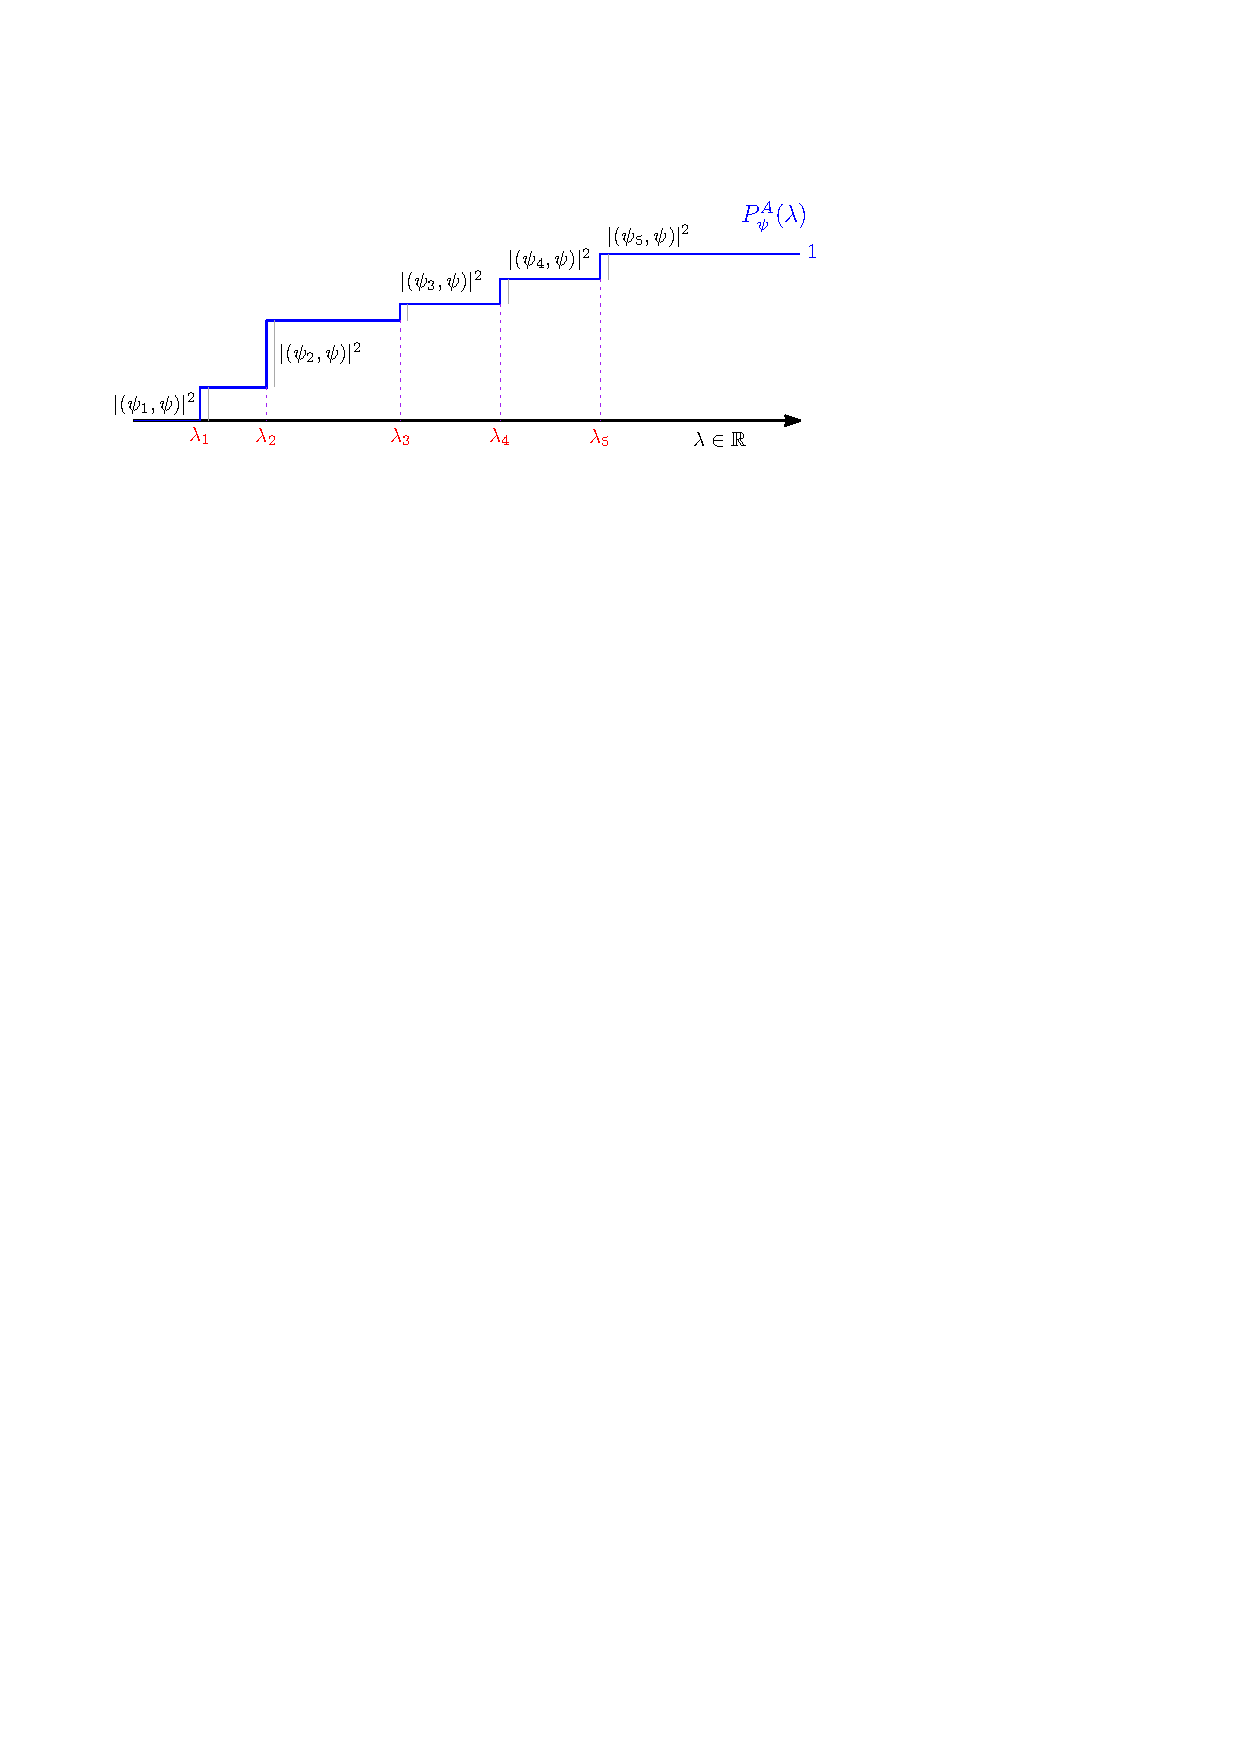
\includegraphics{Immagini/Heaviside.pdf}
    \caption{Andamento di $P_\psi^A(\lambda)$}
    \label{fig:Pautov}
\end{figure}
Supponiamo di porre sulla retta reale gli autovalori, in ordine crescente. In particolare, vi sarà un autovalore minimo $\lambda_1$, prima del quale la $P_\psi^A\left(\lambda\right)$ è nulla. Quando incontra il primo autovalore vi è un \q{gradino} (dato dalla Heaviside), e allo stesso modo per i successivi autovalori, con \q{il salto} tra ciascuno che è dato dal peso $\left|\psi_n,\ \psi\right|^2$, come illustrato in figura \ref{fig:Pautov}.\\
Alla fine (dopo tutti gli autovalori), giungerà ovviamente a $1$, essendo normalizzata la $\psi$ normalizzata: $\norm{\psi}=1$. Perciò:
\[
\sum_{n}\left|(\psi_n,\ \psi\right)|^2=1
\]
In particolare:
\[
P_\psi^A\left(\lambda\right)=\text{ probabilità in una misura di $A$ nello stato $\psi$  di trovare un valore }\leq \lambda 
\]
Perciò costruendo l'operatore $P^A$ grazie alla decomposizione spettrale possiamo ricreare la struttura probabilistica (e in particolare ottenere la \q{probabilità cumulativa} $P^A_\psi$).\\
Elenchiamo ora alcune \textbf{proprietà}\marginpar{Proprietà di $P^A(\lambda)$} degli operatori $\left\{P^A\left(\lambda\right),\ \lambda\in\mathbb{R}\right\}$ dati da $P^A(\lambda) = \sum_n H(\lambda-\lambda_n)P_n$
(siamo sempre nel caso di $\dim{\mathcal{H}}<\infty$). L'idea è di richiedere le stesse proprietà anche nel caso infinito-dimensionale, in modo da svincolarsi dalle equazioni agli autovalori e poter generalizzare.
\begin{enumerate}
    \item $P^A(\lambda)$ è un \textbf{proiettore}\marginpar{$P^A(\lambda)$ è un proiettore}. Infatti è autoaggiunto:
    \[
	\left(\sum_{n}{H\left(\lambda-\lambda_n\right)P_n}\right)^\dag=\sum_{n}{H\left(\lambda-\lambda_n\right)^\ast\ P_n^\dag}=\sum_{n}{H\left(\lambda-\lambda_n\right)P_n}
	\]
	Dove si è usato il fatto che $H$ è reale (quindi pari al suo coniugato), e $P_n$ è autoaggiunto.\\
	Vale anche la seconda condizione per i proiettori, ossia che $P^A(\lambda)^2 = P^A(\lambda)$:
	\begin{equation}
	P^A\left(\lambda\right)^2
	=\left(\sum_{n}{H\left(\lambda-\lambda_n\right)P_n}\right)\left(\sum_{m}{H\left(\lambda-\lambda_m\right)P_m}\right)
	\label{eqn:PAquadro}
	\end{equation}
	Dove si ha che:
	\begin{align*}
	P_nP_m\psi&\underset{(a)}{=}P_n\left(\psi_m,\psi\right)\psi_m \underset{(b)}{=}\left(\psi_m,\psi\right)\left(\psi_n,\psi_m\right)\psi_n \underset{(c)}{=}\\
	&= \delta_{nm}(\psi_m, \psi) \psi_n = 
	\delta_{nm}\underbrace{\braket{\psi_m | \psi}\ket{\psi_n}}_{P_n\psi}  \underset{(d)}{=} 
	P_n\psi\,\delta_{nm}
	\end{align*}
	%[TO DO] \delta_{mn} è una delta di Kronecker, non di Dirac!
	In (a) si applica $P_m$ a $\psi$, che genera $\ket{\psi_m}\braket{\psi_m|\psi}$, mentre in (b) si applica $P_n$ al $\ket{\psi_m}$ appena generato, che porta a $\braket{\psi_n, \psi_m}\ket{\psi_n} \braket{\psi_m|\psi}$. Ma per un operatore simmetrico come $A$ (che è autoaggiunto) possiamo scegliere una base ortonormale di autovettori $\psi_n$, per cui in (c) $\braket{\psi_n|\psi_m} = \delta_{mn}$ (il prodotto scalare restituisce $1$ per la normalizzazione solo quando un vettore è moltiplicato per se stesso, e altrimenti $0$ perché gli autovettori sono ortogonali tra loro). Infine in (d) usiamo la $\delta$ per identificare $n=m$, e riconoscere in $\braket{\psi_m | \psi}\ket{\psi_n}$ il proiettore $P_n$ applicato a $\psi$.\\
	Se consideriamo solo l'operatore \q{puro} avremo perciò $P_n P_m = \hlc{Yellow}{P_n \delta_{nm}}$\\
	Sostituendo questo risultato in (\ref{eqn:PAquadro}):
	\begin{align*}
	P^A(\lambda)^2 &= \sum_{n,m} H(\lambda -\lambda_n)H(\lambda-\lambda_m) \hlc{Yellow}{P_n P_m} = \\
	&= \sum_{n,m}{H\left(\lambda-\lambda_n\right)H\left(\lambda-\lambda_m\right)P_n\delta_{nm}}= \\
	&\underset{(a)}{=} \sum_{n}{H\left(\lambda-\lambda_n\right)H\left(\lambda-\lambda_n\right)P_n}\\
	&\underset{(b)}{=}\sum_{n}{H\left(\lambda-\lambda_n\right)P_n}=P^A\left(\lambda\right)
	\end{align*}
	In (a) abbiamo usato la $\delta$ per identificare $n=m$ e collassare la doppia sommatoria a un'unica variabile.\\
	In (b), invece, si è usato il fatto che la Heaviside assume come valori solo $0$ e $1$, e in particolare è una funzione caratteristica, e il suo quadrato è ovviamente se stessa - in effetti l'avevamo vista come analogo nelle funzioni dei proiettori.
	\item $
	\displaystyle 
	\lim_{\lambda\rightarrow-\infty}{P^A\left(\lambda\right)=0};\quad 
	\lim_{\lambda\rightarrow+\infty}{P^A\left(\lambda\right)}=\sum_{n} P_n=\sum_{n}\left|\psi_n\right\rangle\left\langle\psi_n\right|=\bb{I}
	$\\
	Seguendo\marginpar{Comportamento asintotico di $P^A(\lambda)$} un po' il discorso già fatto per $P_\psi^A(\lambda)$, per $\lambda\to-\infty$ non vi sarà alcun autovalore $\lambda_n \leq \lambda$, e perciò l'operatore darà $0$ (nella definizione, l'Heaviside è costantemente $0$ per $\lambda\to -\infty$). All'estremo opposto, invece, avremo che l'operatore è semplicemente la somma di tutti i proiettori $P_n$ - e la somma di tutte le proiezioni (vettoriali) di un vettore su una base ON è il vettore stesso - da cui l'operatore agisce come l'identità. 
	\item 
	$\displaystyle P^A\left(\lambda\right)P^A\left(\lambda '\right)=P^A\left(\lambda '\right)P^A\left(\lambda\right)=P^A\left(\min{\left\{\lambda,\ \lambda '\right\}}\right) $\\
	Per comprenderlo\marginpar{Composizione di $P^A(\lambda)$} applichiamo la definizione, e concentriamoci sulle Heaviside. In particolare, esaminiamo la seguente espressione nella variabile $\lambda''$:
	\[
	H\left(\lambda-\lambda^{\prime\prime}\right)H(\lambda '-\lambda^{\prime\prime})
	\]
	Il primo termine è $1$ per $\lambda^{\prime\prime}<\lambda$, e il secondo è $1$ solamente se $\lambda^{\prime\prime}<\lambda'$.\\
	Perciò il valore sarà $1$ nell'intersezione tra i due insiemi, che è data da $\lambda^{\prime\prime}<\min{\left\{\lambda,\ \lambda'\right\}}$, e la funzione si può riscrivere come:
	\[
	H\left(\min{\left\{\lambda,\ \lambda '\right\}}-\lambda^{\prime\prime}\right)
	\]
	\item $\displaystyle \lim_{\lambda\rightarrow\lambda_0^+}{P^A\left(\lambda\right)}=P^A(\lambda_0) $\\
	Poiché la Heaviside\marginpar{$P^A(\lambda)$ sono continui a destra} è $1$ in $0$ (è continua da destra, ma non da sinistra), perciò il \q{valore da sopra} è lo stesso della funzione in quel punto. Più precisamente:
	\[
	\lim_{x\rightarrow 0^+}{H \left(x\right)}=1; \quad 
	\lim_{x\rightarrow 0^-}{H\left(x\right)}=0
	\]
\end{enumerate}
\begin{dfn}
Una famiglia di proiettori\marginpar{Famiglia spettrale} $\left\{P\left(\lambda\right),\ \lambda\in\mathbb{R}\right\}$ che soddisfa le proprietà 2-4, è detta \textbf{famiglia spettrale}.
\end{dfn}

\begin{thm}
Esiste una corrispondenza biunivoca\marginpar{Operatore autoaggiunto $\leftrightarrow$ famiglia spettrale} tra operatori autoaggiunti $A=A^\dag$ e famiglie spettrali definita da:
\begin{align}
\nonumber &\left\{P\left(\lambda\right),\lambda\in\mathbb{R}\right\}\rightarrow A\\
D\left(A\right)&= \left\{\phi\in\mathcal{H}\ |\ \int_{\mathbb{R}}{\lambda^2\ d\left(\phi,P\left(\lambda\right)\phi\right)<\infty}\right\} 
\label{eqn:dominiofamigliaspettrale}
\end{align}
Si ha che $D(A)$ è denso, quindi per definire $A$ basta darne gli elementi di matrice:
\[
\left(\phi,A\phi\right)=\int_\bb{R} \lambda\, d\left(\phi,P\left(\lambda\right)\phi\right)
\]
Più in generale, se $f$ è una funzione misurabile su $\bb{R}$, esiste un operatore $f\left(A\right)$ con dominio $D(f(A))$ denso in $\hs$, dato da:
\[
D\left(f\left(A\right)\right)= \left\{\phi\in\mathcal{H}\ |\ \int\left|f\left(x\right)\right|^2d\left(\phi,P\left(\lambda\right)\phi\right)<\infty\right\}
\]
L'operatore $f(A)$ è quindi definito completamente dai suoi elementi di matrice:
\[
\left(\phi,f\left(A\right)\phi\right)=\int f\left(\lambda\right) d(\phi , P\left(\lambda\right)\phi )
\]
(Qui negli elementi di matrice stiamo usando tutti vettori nel dominio denso dell'operatore, poiché abbiamo visto che è possibile utilizzare l'\textbf{identità di polarizzazione} per riscrivere il tutto in termini di valori medi)
\end{thm}
\textbf{Dim.} (molto tecnica e lunga, omessa)\\
In particolare, per la speciale funzione $H(\lambda-A)$ si ha:
\[
H(\lambda-A) = P(\lambda)
\]
(per chiarire, prova a pensare tutto ciò in termini di spazi finito-dimensionali).\\
Con questa strategia non abbiamo usato autovettori/autovalori, e perciò tramite questa è possibile estendere quanto detto nel caso finito-dimensionale all'infinito-dimensionale.

\textbf{Esempio}\index{Famiglia spettrale!operatore posizione $X$} \marginpar{Esempio (1) di famiglia spettrale: operatore posizione}
In $\hs =L^2(\bb{R}, dx)$, consideriamo la \textbf{famiglia spettrale}:
\begin{equation}
\left(P\left(\lambda\right)\psi\right)\left(x\right)=H\left(\lambda-x\right)\psi \left(x\right)
\label{eqn:famiglia_spettrale_x}
\end{equation}
Verifichiamo che soddisfa tutte le proprietà:
\begin{enumerate}
    \item $H$ reale e $H^2=H$, quindi è un proiettore.
    \item 
    $\displaystyle \lim_{\lambda\rightarrow-\infty}{H\left(\lambda-x\right)\psi\left(x\right)=0};
    \quad
	\lim_{\lambda\rightarrow+\infty}{H\left(\lambda-x\right)\psi(x)}=\psi
	\left(x\right)\>\forall \psi \in \hs $
    \item 
    $\displaystyle H\left(\lambda-x\right)H\left(\lambda '-x\right)=H\left(\min{\left\{\lambda,\ \lambda '\right\}}-x\right)$
    \item 
    $\displaystyle \lim_{\lambda\rightarrow\lambda_0^+}{H\left(\lambda-x\right)}=H\left(\lambda_0-x\right)$
\end{enumerate}
Di quale operatore autoaggiunto è la famiglia spettrale? Calcoliamone il dominio:
\begin{align*}
D\left(A\right)&= \left\{\phi\in L^2\left(\mathbb{R}\right)\ |\ \int_\bb{R}\lambda^2\, d\left(\phi,P\left(\lambda\right)\phi\right)<\infty\right\}\\
\left(\phi,P\left(\lambda\right)\phi\right)&=\int_\bb{R} dx\, \phi^\ast\left(\lambda\right)H\left(\lambda-x\right)\phi \left(x\right)\\
d\left(\phi,P\left(\lambda\right)\phi\right)&=\left(\int_\bb{R} dx\,\phi^\ast\left(x\right)\delta\left(\lambda-x\right)\phi\left(x\right)\right)d\lambda =\phi^\ast\left(\lambda\right)\phi \left(\lambda\right)d\lambda 
\end{align*}
E quindi:
\begin{align*}
D\left(A\right)&= \left\{\phi\in L^2\left(\mathbb{R},dx\right)\ \ |\ \ \int\lambda^2\phi^\ast\left(\lambda\right)\phi\left(\lambda\right)\,d\lambda<\infty\right\}= \left\{\left|\left|x\phi\right|\right|^2<\infty\right\}
\end{align*}
E gli elementi di matrice sono dati da:
\begin{align*}
    \left(\phi,A\phi\right)=\int \lambda\, d\left(\phi,P\left(\lambda\right)\phi\right)= \int \lambda\,\phi^\ast\left(\lambda\right)\phi \left(\lambda\right)d\lambda =\int x\,\phi^\ast\left(x\right)\phi \left(x\right)dx
\end{align*}
Riconosciamo l'azione dell'operatore \textbf{posizione}:
\begin{align*}
    X\phi \left(x\right)&=x\,\phi \left(x\right)\\
    D\left(X\right)&=\left\{\phi\in L^2\ |\ \left|\left|x\phi\right|\right|^2<\infty\right\}
\end{align*}
Quindi $A=X$, e $dP_\phi^X(\lambda) = |\phi(\lambda)|^2 d\lambda$.\\
Se $\phi$  non è normalizzato, perché sia \[ \int_{\mathbb{R}}{dP_\phi^X\left(\lambda\right)}=1 \]
Bisogna scrivere:
\[
dP_\phi^X\left(\lambda\right)=\hlc{SkyBlue}{\frac{\left|\phi\left(\lambda\right)\right|^2}{\left|\left|\phi\right|\right|^2}}d\lambda 
\]
La grandezza evidenziata in azzurro è la \textbf{densità di probabilità}\marginpar{Densità di probabilità} che misurando $X$ nello stato $\phi$ si ottenga $\lambda$. In fisica si denota con:
\[
w_\phi^X\left(\lambda\right)=\frac{dP_\phi^X\left(\lambda\right)}{d\lambda}=\frac{\left|\phi\left(\lambda\right)\right|^2}{\left|\left|\phi\right|\right|^2}
\]
Il valor medio è quindi:
\[
\left\langle X\right\rangle_\phi=\int \lambda  dP_\phi^X\left(\lambda\right)=\int \lambda  w_\phi^X\left(\lambda\right) d\lambda 
\]
Riepilogando: \marginpar{Riepilogo delle \textbf{proprietà} delle \textbf{osservabili}}
\begin{enumerate}
    \item Le osservabili sono \textbf{operatori} $A$ e dalla indipendenza del rappresentativo del raggio vettore nel calcolo dei valor medi $\langle A\rangle_\psi$ si ha che $A$ sono \textbf{lineari} (e richiediamo abbiano un dominio denso in $\hs$, ossia il più largo possibile).
    \item Vogliamo poi che $\langle A \rangle_\psi \in \bb{R}$, da cui $A$ deve essere \textbf{simmetrico}.
    \item La richiesta che esista $f\left(A\right)$ implica che $A$ è \textbf{autoaggiunto}.  Ciò consente anche di costruire una interpretazione probabilistica, potendo definire la funzione $P_\psi^A\left(\lambda\right)$
\end{enumerate}
Enunciamo questi risultati, che abbiamo costruito nei paragrafi precedenti e che sono estensivamente corroborati dall'evidenza, come \textbf{assiomi} del formalismo quantistico.
\begin{axi}
Le \textbf{osservabili}\marginpar{Assioma delle osservabili}\index{Assioma!delle osservabili} di un sistema quantistico, i cui \textbf{stati puri} sono descritti dai \textbf{raggi vettori} di $\hs$, sono descritti da \textbf{operatori autoaggiunti} $A=A^\dag$ in $\hs$.
\end{axi}

\begin{axi}
La \textbf{probabilità}\marginpar{Assioma della probabilità}\index{Assioma!della probabilità} che il risultato di una misura di $A$ nello stato $\psi$ (ricavata ripetendo tante volte la misura sperimentale nelle stesse condizioni) sia in $]-\infty , \lambda]$ è data da:
\[
P_\psi^A\left(\lambda\right)=\frac{(\psi,\ P^A\left(\lambda\right)\psi)}{\norm{\psi}^2}
\]
Dove $P^A\left(\lambda\right)$ è la \textbf{famiglia spettrale} di $A$ e $\forall \psi \in D\left(A\right)$:
\[
\langle A \rangle_\psi = \frac{(\psi, A\psi)}{\norm{\psi}^2}
\]
\end{axi}

\subsection{Osservazioni sulle proprietà matematiche delle osservabili}
\begin{enumerate}
    \item La condizione di autoaggiuntezza è delicata: 
	Ad esempio, se $A$ e $B$ sono autoaggiunti \textbf{limitati}, $A+B$ lo è, ma $AB$ no. Infatti $\left(AB\right)^\dag=B^\dag A^\dag=BA\neq AB$.\\
	Perciò gli operatori autoaggiunti non formano un'algebra sui reali.\\
	Possiamo costruire un'algebra degli operatori autoaggiunti su $\bb{C}$, e in effetti $\frac{\left(AB-BA\right)}{i}$ è autoaggiunto.
	\item Se invece $A$ e $B$ sono autoaggiunti, ma \textbf{illimitati} in $D\left(A\right)$ e $D(B)$ densi in $\hs$. Allora $(A+B)$ è ben definito in $D\left(A\right)\cap D\left(B\right)$ ma $A+B$ in generale non è autoaggiunto in $D\left(A\right)\cap D\left(B\right)$ che potrebbe addirittura non essere denso.\\
	Questo problema appare in fisica ad esempio per l'osservabile energia:
	\[
	H=\frac{{\vec{p}}^{\,2}}{2m}+V(\vec{x})
	\]
	Con $A=\frac{{\vec{p}}^2}{2m}, B=V(\vec{x})$\\
	Fortunatamente, molti casi importanti sono coperti dal seguente risultato:
	\begin{thm}
	Se $V$ è limitato in $\mathbb{R}^n$, oppure se $n=3$ e $V$ è Coulombiano (es. potenziale elettrostatico), allora $H$ è autoaggiunto nel dominio di $A$ definito da:
	    \[
	    D\left(\vec{p}^{\>2}\right)=\left\{\varphi\in L^2\left(R^n,\ d^nx\right)\middle|\ {\vec{p}}^{\>2}\widetilde{\varphi}\left(\vec{p}\,\right)\in L^2\left(R^n, d^np\right)\right\}
	    \]
	\end{thm}
	\item \textbf{Attenzione}: Conoscere $\sigma(A)$ e $\sigma(B)$ non porta alla conoscenza di $\sigma(A+B)$.\\
	Per esempio, $A=\frac{p^2}{2m}, B=V\left(x\right)$, con $\sigma \left(A\right)= \mathbb{R}_+, \sigma \left(V\left(x\right)\right)=\op{cod} V(x)$ sono entrambi operatori a spettro continuo. Tuttavia la loro somma contiene uno spettro discreto: sono per esempio i livelli energetici di una buca infinita.\\
	(In \MC, d'altro canto, conoscere $\sigma(A)$ e $\sigma(B)$ porta subito alla conoscenza di $\sigma(A+B)$.)\\
\end{enumerate}
\end{document}

%16_10a
\documentclass[../../FisicaTeorica.tex]{subfiles}

%%%PACKAGES
\usepackage[usenames, dvipsnames, table]{xcolor}
\usepackage[utf8]{inputenc}
\usepackage[T1]{fontenc}
\usepackage{lmodern}
\usepackage{amsmath}
\usepackage{amsthm}
\usepackage{amsfonts}
\usepackage{comment}
\usepackage{wrapfig}
\usepackage{booktabs}
\usepackage{braket}
\usepackage{pgf,tikz}
\usepackage{mathrsfs}
\usetikzlibrary{arrows}
\usepackage{subfigure}
\usepackage{xspace}
\usepackage{gnuplottex}
\usepackage{epstopdf}
\usepackage{marginnote}
\usepackage{float}
\usetikzlibrary{tikzmark}
\usepackage{graphicx}
\usepackage{cancel}
\usepackage{bm}
\usepackage{mathtools}
\usepackage{hyperref}
\usepackage{ragged2e}
\usepackage[stable]{footmisc}
\usepackage{enumerate}
\usepackage{mathdots}
\usepackage[framemethod=tikz]{mdframed}
\PassOptionsToPackage{table}{xcolor}
\usepackage{soul}
\usepackage{enumerate}
\usepackage{mathdots}
\usepackage[framemethod=tikz]{mdframed} %Added 16/10
\usepackage[italian]{babel} %Added 16/10
\usepackage{amssymb} %Added
\usepackage{enumitem}
\usepackage{array}


%%BOOKTAB
\setlength{\aboverulesep}{0pt}
\setlength{\belowrulesep}{0pt}
\setlength{\extrarowheight}{.75ex}
\setlength\parindent{0pt} %Rimuove indentazione


%%GEOMETRIA
\usepackage[a4paper]{geometry}
 \newgeometry{inner=20mm,
            outer=49mm,% = marginparsep + marginparwidth 
                       %   + 5mm (between marginpar and page border)
            top=20mm,
            bottom=25mm,
            marginparsep=6mm,
            marginparwidth=30mm}
\makeatletter
\renewcommand{\@marginparreset}{%
  \reset@font\small
  \raggedright
  \slshape
  \@setminipage
}
\makeatother
 

%%COMANDI
\newcommand{\q}[1]{``#1''}
\newcommand{\lamb}[2]{\Lambda^{#1}_{\>{#2}}}
\newcommand{\norm}[1]{\left\lVert#1\right\rVert}
\newcommand{\hs}{\mathcal{H}}
\newcommand{\minus}{\scalebox{0.75}[1.0]{$-$}}
\newcommand{\hlc}[2]{%
  \colorbox{#1!50}{$\displaystyle#2$}}
\newcommand{\bb}[1]{\mathbb{#1}}
\newcommand{\op}[1]{\operatorname{#1}}
\renewcommand{\figurename}{Fig.}
\newcommand{\dom}[1]{D#1}
\newcommand{\avg}[1]{\left\langle{#1}\right\rangle}
\newcommand{\NN}{\mathbb N}
\newcommand{\RR}{\mathbb R}
\newcommand{\CC}{\mathbb C}
\newcommand{\mS}{\mathcal S}
\newcommand{\de}{d}
\newcommand{\abs}[1]{\left|#1\right|}

\newcommand{\lesson}[2]{\marginpar{(Lezione #1 del #2)}}
\DeclareRobustCommand{\MQ}{{\small\textsc{MQ}}\xspace}
\DeclareRobustCommand{\MC}{{\small\textsc{MC}}\xspace}
%Prima era \small\textsc{MQ}\xspace

%%TESTATINE
\usepackage{fancyhdr}
\pagestyle{fancy}
\fancyhead{} % clear all header fields
\renewcommand{\headrulewidth}{0pt} % no line in header area
\fancyfoot{} % clear all footer fields
%\fancyfoot[R]{A.A. 2018/19} % other info in "inner" position of footer line
\cfoot{\thepage}


%%AMBIENTI
\theoremstyle{plain}
\newtheorem{thm}{Teorema}[section]
\newtheorem{lem}{Lemma}[section]
\newtheorem{prop}{Proposizione}[section]
\newtheorem{axi}{Assioma}
\newtheorem{pst}{Postulato}

\theoremstyle{definition}
\newtheorem{dfn}{Definizione}

\theoremstyle{remark}
\newtheorem{oss}{Osservazione}
\newtheorem{es}{Esempio}
\newtheorem{ex}{Esercizio}

%Spiegazioni/verifiche
\newenvironment{expl}{\begin{mdframed}[hidealllines=true,backgroundcolor=green!20,innerleftmargin=3pt,innerrightmargin=3pt,leftmargin=-3pt,rightmargin=-3pt]}{\end{mdframed}} %Box di colore verde

\newenvironment{appr}{\begin{mdframed}[hidealllines=true,backgroundcolor=blue!10,innerleftmargin=3pt,innerrightmargin=3pt,leftmargin=-3pt,rightmargin=-3pt]}{\end{mdframed}} %Approfondimenti matematici (box di colore blu)

%%Domande di Marchetti
\newtheorem{question}{Domanda}


%%OPERATORI
\DeclareMathOperator{\sech}{sech}
\DeclareMathOperator{\csch}{csch}
\DeclareMathOperator{\arcsec}{arcsec}
\DeclareMathOperator{\arccot}{arcCot}
\DeclareMathOperator{\arccsc}{arcCsc}
\DeclareMathOperator{\arccosh}{arcCosh}
\DeclareMathOperator{\arcsinh}{arcsinh}
\DeclareMathOperator{\arctanh}{arctanh}
\DeclareMathOperator{\arcsech}{arcsech}
\DeclareMathOperator{\arccsch}{arcCsch}
\DeclareMathOperator{\arccoth}{arcCoth} 




\begin{document}
%\subsection{Quali operatori rappresentano osservabili in \MQ?}
Riepilogando: abbiamo visto che $A$ deve essere lineare, di dominio denso, simmetrico (valor medi reali), e se vogliamo che esistano funzioni $f(A)$, si ha:
\begin{equation}
    \langle A \rangle_\psi = \int \lambda \, dP_\psi^A(\lambda) \Rightarrow A=A^\dag
    \label{eqn:autoadjoint}
\end{equation}
\begin{oss}
Sia\marginpar{$e^{iaA}$ è un operatore unitario} $f\left(\lambda\right)=e^{i\lambda a}, a\in \bb{R}$. Applicandola ad un operatore generico otteniamo, formalmente, $f(A) = e^{iaA}$. Dimostriamo che il nuovo operatore $f(A)$ è unitario.\\ Nella notazione formale di (\ref{eqn:operatoreformale}) si ha che:
\[
f(A) = e^{iaA} = \int e^{iaA} dP^A(\lambda)
\]
Calcolandone l'aggiunto:
\begin{equation}
\left(e^{iaA}\right)^\dag=\left(\int e^{ia\lambda}dP^A\left(\lambda\right)\right)^\dag
\underset{(a)}{=}\int e^{-ia\lambda}dP^A\left(\lambda\right)\underset{(b)}{=}e^{-iaA}=\left(e^{iaA}\right)^{-1}
\label{eqn:esponenzialeunitario}
\end{equation}
dove in (a) si è usato il fatto che $dP^A(\lambda)$ è autoaggiunto, e perciò l'unico cambiamento sta nel prendere il complesso coniugato dell'esponenziale. Riconosciamo allora in (b) la funzione $g(A) = e^{-iaA}$ scritta nel formalismo di (\ref{eqn:operatoreformale}), che è esattamente l'inversa di $f$, e ciò rende $f(A)$ un operatore unitario.
\label{dim:esponenzialeunitario}
\end{oss}
\begin{oss}
Dato un vettore in notazione di Dirac $\ket{\phi}$ il proiettore $P_\phi =\ket{\phi}\bra{\phi}$ è autoaggiunto, quindi descrive un'osservabile (per la corrispondenza biunovica tra autoaggiunti e famiglie spettrali), che corrisponde alla domanda: il sistema si trova nello stato $\ket{\phi}$?\\
Il valor medio di $\ket{\phi}\bra{\phi}$ nello stato $\ket{\psi}$ è infatti dato da (assumendo stati normalizzati, con $\braket{\phi|\phi} = 1 = \braket{\psi|\psi}$):
\[
(\psi, P_\phi \psi) = 
\braket{\psi|\phi}\braket{\phi|\psi} = |\braket{\psi|\phi}|^2
\]
che viene detto \textbf{probabilità di transizione}\marginpar{Probabilità di transizione} (e $\braket{\psi|\phi}$ ampiezza di transizione) da $\ket{\phi}$ a $\ket{\psi}$.\\
Poiché tale probabilità è non nulla anche per $\ket{\phi}\neq\ket{\psi}$ (anche come raggi vettori), vediamo che in \MQ \textbf{gli stati puri non sono mutualmente esclusivi}, come invece avviene nel caso classico,\marginpar{Stati puri distinti non sono mutualmente esclusivi} in cui o due punti (intesi nello spazio delle fasi $\Omega$) coincidono o sono distinti.\\
In \MQ, dando l'analogo delle condizioni iniziali (vettore nello spazio di Hilbert, stato puro = massima informazione), provando a fare una misura in generale posso ottenere il risultato di uno stato diverso. Alternativamente, se preparo il sistema ad un istante $t=0$ nello $\ket{\phi}$, a $t=0^+$ è possibile trovarlo nello stato $\ket{\psi}\neq\ket{\phi}$!\\
Matematicamente ciò è dato dal fatto che due generici vettori, se moltiplicati scalarmente, non sempre devono dare un risultato nullo - tale ovvietà produce un risultato fisico per nulla intuitivo.\\
Del resto, in \MC gli stati puri sono costituiti da delta di Dirac, e il prodotto di due $\delta$ diverse è per forza nullo.
\end{oss}
\textbf{Esercizio}.\marginpar{Esempio (2) di famiglia spettrale: il momento} Si consideri la famiglia di operatori $\left\{P\left(\lambda\right),\ \lambda\in\mathbb{R}\right\}$ definiti in $L^2\left(\mathbb{R},\ dx\right)$ da:
\[
\left(P\left(\lambda\right)\psi\right)\left(x\right)=\frac{1}{2\pi\hbar}\int_{\mathbb{R}}{\left(\int_{-\infty}^{\lambda}e^{i\frac{p}{\hbar}\left(x-x'\right)}dp\right)\psi\left(x'\right)dx'}
\]
Si dimostri che $P\left(\lambda\right)$ è una \textbf{famiglia spettrale} (solo il fatto che $P\left(\lambda\right)$ sono proiettori) e si trovi la corrispondente osservabile.\\

Verifichiamo innanzitutto l'autoaggiuntezza, ossia che: $\left(P\left(\lambda\right)\right)^\dag=P\left(\lambda\right)$
Partendo dagli elementi di matrice:
\[
\left(\phi,P\left(\lambda\right)\psi\right)=\left(P^\dag\left(\lambda\right)\phi,\psi\right)
\]
Svolgendo il prodotto scalare, il primo termine è pari a:
\begin{align*}
(\phi, P(\lambda)\psi) &= \int{\phi^*\left(x\right)}\int{\frac{1}{2\pi\hbar}\left(\int_{-\infty}^{\lambda}{e^{i\frac{p}{\hbar}\ \left(\bm{x-x'}\right)}\ }dp\right)\psi\left(x'\right)dx' d x}=\\
&={\int\limits{\left(\frac{1}{2\pi\hbar}\int_{-\infty}^{\lambda}{\exp\left({i\frac{p}{\hbar}\left(\bm{x'-x}\right)}\right )dp\ \phi\left(x\right)dx}\right)}}^*\psi \left(x'\right)dx'
\end{align*}
dove si è \q{\textit{spostata l'azione dell'operatore al primo membro del prodotto scalare}}, portando tutto ciò che dipenda da $x$ sotto lo stesso segno di integrale ed evidenziando una coniugazione complessa (si noti il cambio di segno nell'esponenziale).\\
Possiamo ora notare che il termine tra parentesi è l'azione di $P^\dag (\lambda)$ su un $\phi$:
\begin{align*}
    \left(P^\dag\left(\lambda\right)\phi\right)\left(x'\right)=\frac{1}{2\pi\hbar}\int{\left(\int_{-\infty}^{\lambda}{\exp\left ({i\frac{p}{\hbar}\left(x'-x\right)}\right )dp}\right)\phi\left(x\right)dx=\left(P\left(\lambda\right)\phi\right)(x')}
\end{align*}
Dimostriamo quindi che $P$ è un proiettore, e cioè che $P^2\left(\lambda\right)=P\left(\lambda\right)$. La cosa non è immediata - ci servirà passare in una notazione più conveniente. Notando la presenza di esponenziali e integrali nella definizione di $P$, un'idea è di sfruttare le trasformate di Fourier\footnote{In effetti da Fisica Moderna possiamo già intuire che questo operatore sia l'operatore momento, che è ricavato a partire dall'operatore posizione tramite trasformate di Fourier}\\
Osserviamo che se definiamo trasformata e antitrasformata di Fourier come:
\begin{align*}
\left(\mathcal{F}\psi\right)\left(p\right)&\equiv\frac{1}{\sqrt{2\pi\hbar}}\int_{\mathbb{R}}
{\exp\left (\bm{-}{i\frac{p}{\hbar}x}\right )\psi\left(x\right)dx\ } = \widetilde{\psi}\left(p\right)\\
(\mathcal{F}^{-1}\tilde{\psi})(x) &\equiv  \frac{1}{\sqrt{2\pi\hbar}}\int_\bb{R} \exp\left(i\frac{p}{\hbar}x\right) \tilde{\psi}(p)\, dp
\end{align*}
Possiamo riscrivere $(P(\lambda)\psi)(x)$ tramite trasformate di Fourier, e quindi usare le proprietà di queste ultime per dimostrare $P=P^2$. Partiamo dall'azione di $P(\lambda)$ su $\psi$:
\[
(P(\lambda)\psi)(x') = \int_\bb{R}\left[\frac{1}{2\pi \hbar} \int_{-\infty}^\lambda \exp\left (i\frac{p}{\hbar}(x'-x)\right )dp\right ]\psi(x) dx
\]
Notiamo che l'integrale \q{esterno} su $x$ è un \textit{integrale di convoluzione}, in quanto ha la struttura di:
\[
(f*g) = \int_\bb{R} f(x)g(x'-x)\,dx
\]
dove la $f(x) = \psi(x)$, e per la $g(x'-x)$ (che corrisponde al termine tra parentesi quadre, ossia all'integrale in $p$), riconosciamo la struttura di un'antitrasformata di Fourier, con due differenze chiave: un fattore $\sqrt{2\pi\hbar}$ in più e un dominio \q{troppo stretto} (non tutto $\bb{R}$).\\
Per quanto riguarda il fattore basta tenerne conto, mentre per correggere il dominio passiamo ad un integrale su tutto $\bb{R}$, e annulliamo il suo valore fuori dalla regione che ci interessa moltiplicando la funzione integranda per l'opportuna funzione di Heaviside $H(\lambda-p)$.\\
Possiamo quindi riscrivere:\footnote{Rinominando la variabile $x'$ con $x$ per comodità}:
\begin{align*}
\left(P\left(\lambda\right)\psi\right)\left(x\right)
&=
\int_\bb{R} \left [\frac{1}{\sqrt{2\pi\hbar}}\int_{-\infty}^{+\infty}\frac{H\left(\lambda-p\right)}{\sqrt{2\pi\hbar}}\exp\left (+{i\frac{p}{\hbar}(x-x')}\right)\ dp\right ]\psi\left(x'\right)dx'=\\
&=\mathcal{F}^{-1}\left(\frac{H\left(\lambda-p\right)}{\sqrt{2\pi\hbar}} \right )*\ \psi\left(x\right)
\end{align*}
Sfruttando \q{al contrario} la proprietà delle trasformate\footnote{Il fattore $1/\sqrt{2\pi\hbar}$ compare perché stiamo usando la \q{normalizzazione angolare} per le trasformate di Fourier}:
\[
\mathcal{F}^{-1}(\phi \psi) =\frac{1}{\sqrt{2\pi\hbar}} \mathcal{F}^{-1}(\phi) * \mathcal{F}^{-1}(\psi)
\]
Otteniamo:
\begin{align*}
(P(\lambda)\psi)(x) &= \mathcal{F}^{-1}\left ( \frac{H(\lambda-p)}{\sqrt{2\pi\hbar}}\right ) * \psi(x) = 
\mathcal{F}^{-1}\left (\frac{H(\lambda-p)}{\sqrt{2\pi\hbar}}\right ) * \mathcal{F}^{-1}(\mathcal{F}\psi)(x) =\\
&= \frac{1}{\sqrt{2\pi\hbar}} \mathcal{F}^{-1}(H(\lambda-p)*\mathcal{F}^{-1}(\mathcal{F}\psi)(x) 
= \mathcal{F}^{-1}(H(\lambda-p)\mathcal{F}\psi)
\end{align*}
(dove si è usata la linearità dell'antitrasformata per portar fuori il fattore di normalizzazione $1/\sqrt{2\pi\hbar}$).\\
%Aggiungi passaggio di estrazione del fattore per linearità
Definendo:
\[
\phi(x) = (P(\lambda)\psi)(x) = \mathcal{F}^{-1}(H(\lambda-p)\mathcal{F}\psi)(x)
\]
Si ha che applicando $P(\lambda)$ a $\phi$ otteniamo $(P(\lambda)^2\psi)(x)$. Facendo allora il conto:
\begin{align*}
    (P(\lambda)\phi)(x) &= \mathcal{F}^{-1}(H(\lambda-p)\mathcal{F}\phi)(x) =\\
    &= \mathcal{F}^{-1}[H(\lambda-p) \mathcal{F}\mathcal{F}^{-1}(H(\lambda-p)\mathcal{F}\psi)](x) =\\
    &\underset{(a)}{=} \mathcal{F}^{-1}(H(\lambda-p)H(\lambda-p)\mathcal{F}\psi)(x) =\\
    &\underset{(b)}{=} \mathcal{F}^{-1}(H(\lambda-p)\mathcal{F}\psi)(x) = (P(\lambda)\psi)(x)
\end{align*}
In (a) si è sfruttata la proprietà di Fourier, per cui trasformata e antitrasformata sono una l'inversa dell'altra (e la loro composizione è l'identità). Per (b), invece, basta notare che $H(\lambda-p)$ ha come valori solo $1$ e $0$ (in particolare è la funzione caratteristica di $]-\infty, \lambda]$) e quindi è pari al suo quadrato (come si era visto tra gli esempi di \q{funzioni unitarie}).\\
Avendo quindi dimostrato che $P$ è autoaggiunto e $P=P^2$ si ha che $P$ è un proiettore.\\
Si può verificare (ma non lo faremo) che i $P(\lambda)$, $\lambda \in \bb{R}$ costituiscono una \textit{famiglia spettrale} (cioè soddisfano anche le altre tre proprietà che abbiamo elencato). Ogni famiglia spettrale è associata ad un'osservabile: esaminiamola.
Sia $\ket{\psi}$ normalizzata ($\braket{\psi|\psi} = 1$). Il valor medio dell'operatore $A$ associato alla famiglia spettrale $P(\lambda)$ nello stato $\psi$ è dato da:
\begin{equation}
\langle A \rangle_\psi = \int \lambda d(\psi, P(\lambda)\psi)
\label{eqn:valormediop}
\end{equation}
Espandendo il prodotto scalare: 
\begin{align*}
&d\left(\psi,P\left(\lambda\right)\psi\right)=d_\lambda\int \int \psi^*\left(x\right)
\left ( \int_{-\infty}^{\bm{\lambda}}\frac{e^{i\frac{p}{\hbar}\left(x-x'\right)}}{2\pi\hbar}\ dp\right )
\psi\left(x'\right)dx\ dx'=\\
&\underset{(a)}{=}\left[\int\int\psi^*\left(x\right)
\exp \left ({i\frac{\lambda}{\hbar}\left(x-x'\right)}\right ) \frac{1}{2\pi\hbar}\ \psi\left(x'\right)dx\ dx'\right]d\lambda =\\
&\underset{(b)}{=} \underbrace{\left [ \frac{1}{\sqrt{2\pi\hbar }}\int_\bb{R} \left ( \psi(x) \exp \left (-i\frac{\lambda}{\hbar}x\right )\right )^*dx \right ]}_{(\mathcal{F}\psi)^*(\lambda)}
\cdot 
\underbrace{\left [ \frac{1}{\sqrt{2\pi\hbar}} \int_\bb{R} \psi(x') \exp\left (-i\frac{\lambda}{\hbar}x'\right )dx' \right ]}_{(\mathcal{F}\psi)(\lambda)}
d\lambda =\\
&= \left(\mathcal{F}\psi\right)^*\left(\lambda\right)\left(\mathcal{F}\psi\right)\left(\lambda\right)d\lambda=\left|\widetilde{\psi}\left(\lambda\right)\right|^2d\lambda 
\end{align*}
In (a) notiamo che la derivata per $\lambda$ agisce solo sull'integrale, e per il teorema fondamentale del calcolo restituisce la funzione integranda calcolata in $p = \lambda$. In (b) abbiamo \q{spezzato} l'esponenziale in due fattori, dove si riconosce la struttura delle trasformate di Fourier. Il prodotto di una trasformata per la sua complessa coniugata dà allora il modulo quadro.\\
Sostituendo questo risultato in (\ref{eqn:valormediop}):
\[
\langle A \rangle_\psi = \int \lambda\, |\tilde{\psi}(\lambda)|^2\, d\lambda
\]
Possiamo finalmente calcolare il dominio di $A$, completandone la definizione (facendo riferimento al teorema in (\ref{eqn:dominiofamigliaspettrale})):
\begin{align*}
D\left(A\right)&= \left\{\psi\in L^2\ |\ \int\lambda^2\, \hlc{Yellow}{d\left(\psi,P\left(\lambda\right)\psi\right)}<\infty\right\}=\\
&=\left\{\psi\in L^2\ |\ \int\lambda^2 \hlc{Yellow}{|\widetilde{\psi}\left(\lambda\right)|^2}\,d\lambda<\infty\right\} 
\end{align*}
Se ora esaminiamo:
\begin{equation}
\mathcal{F}\left(-i\hbar\frac{d}{dx}\psi\right)\left(p\right)=\frac{1}{\sqrt{2\pi\hbar}}\int_\bb{R} \exp\left (-i\frac{p}{\hbar}x\right )\left(-i\hbar\frac{d}{dx}\psi\left(x\right)\right)dx 
\label{eqn:trasformatap}
\end{equation}
La condizione imposta nel determinare il dominio fa sì che $\psi \left(x\right)\xrightarrow[x\to \infty]{} 0$ (lo dimostreremo più avanti in un altro esempio). Ciò significa che \textbf{integrando per parti} il primo termine (che viene valutato tra $-\infty$ e $\infty$) si annulla, e perciò lo trascuriamo. Svolgendo quindi i conti rimanenti:
\begin{align*}
(\ref{eqn:trasformatap}) &= \cancel{-}\frac{1}{\sqrt{2\pi\hbar}}\int_\bb{R} \cancel{-}i\hbar \psi(x) \frac{d}{dx}\left(\exp\left(-i\frac{p}{\hbar}x\right)\right)dx =\\
&= \frac{1}{\sqrt{2\pi\hbar}} \int_\bb{R} \hlc{Yellow}{i} \hlc{SkyBlue}{\hbar} \psi(x) \left(\hlc{Yellow}{-i}\frac{p}{\hlc{SkyBlue}{\hbar}}\exp\left ( -i\frac{p}{\hbar}x\right ) \right )dx=\\
&= p\,\underbrace{\frac{1}{\sqrt{2\pi\hbar}}\int_\bb{R}\exp\left(-i\frac{p}{\hbar}x\right ) \psi(x) dx}_{\tilde{\psi}(p)} = p\,\tilde{\psi}(p)
\end{align*}
Ciò significa che la rappresentazione in posizioni e quella in momenti sono collegate da una trasformata di Fourier. Infatti vale, per il teorema di Plancherel\footnote{Il teorema di Plancherel enuncia che una trasformazione di Fourier è un'isometria rispetto alla norma di $L^2$ - e, visto che norma e prodotto scalare sono collegati dall'identità di polarizzazione - anche rispetto al prodotto scalare di $L^2$. In altre parole, il prodotto scalare tra due elementi di $L^2$ dà lo stesso risultato se fatto tra le trasformate di quei due elementi. Qui nello specifico si ha $(\tilde{\psi},A\tilde{\psi}) = (\psi, A_x \psi)$, dove $A=p$ (operatore momento in rappresentazione dei momenti), e $A_x = -i\hbar \frac{d}{dx} = \mathcal{F}(A)$ è lo \q{stesso operatore} in rappresentazione di posizioni.}:
\[
\langle A \rangle_\psi = \int \tilde{\psi}(p)^*\,p\,\tilde{\psi}(p) dp= \int \psi(x)^* \left ( -i\hbar \frac{d}{dx} \psi(x) \right ) dx
\]
Perciò l'operatore $A$ in $D(A)$, usando la rappresentazione in posizioni, è dato da:
\[
A = -i\hbar \frac{d}{dx}
\]

\section{Spettro di un operatore}
Ci poniamo ora il problema di determinare quali valori si possono ottenere con una misura di un operatore autoaggiunto $A=A^\dag$ (o meglio, dell'osservabile da esso descritto).\\
Nel caso $\dim{\mathcal{H}}<\infty$ si ha che $\sigma \left(A\right)= \left\{\lambda_n\text{ autovalori}\right\}$, analogamente al caso classico, dove un'osservabile è data da una funzione $f(q,p)$ i cui valori sono tutti autovalori ($\op{cod} f = \{\text{autovalori di }f\}$).\\
Tuttavia, per $\dim{\mathcal{H}}=\infty$, sorgono fin da subito dei problemi.  Infatti, un autovalore è definito come:
\[
\left(\Delta O\right)_{\lambda,\psi_\lambda}=0 = \norm{(A-\lambda)\psi_\lambda}^2
\]
Con $\psi_\lambda$ autovettore di autovalore $\lambda$ 
(l'equivalenza tra le due scritture è stata ricavata in (\ref{eqn:fluttuazione-autoaggiunto})).\\
Proviamo a imporre tale condizione per trovare gli autovalori dell'operatore \textbf{posizione} su $\bb{R}$ $X\psi \left(x\right)=x\psi (x)$:
\[
\left\langle\left(X-a\right)^2\right\rangle_\psi=\int \left(x-a\right)^2\left|\psi\left(x\right)\right|^2dx=0\Rightarrow \left(x-a\right)^2\psi \left(x\right)=0\Rightarrow  \psi \left(x\right)=0 
\]
(un integrale di quantità positive è nullo se e solo se la funzione integranda è nulla, a meno di insiemi Lebesgue-trascurabili, e perciò in ogni caso corrisponde alla funzione $f\equiv 0$ in $L^2$, considerata come classe di equivalenza).\\
Poiché l'unico risultato è la funzione nulla, ciò significa che in $L^2$ non esiste alcun autovalore diverso da $0$. Fisicamente vuol dire che non esiste la possibilità di localizzare una particella in un punto in \MQ, e matematicamente che:
\[
\nexists\> \psi_n\>|\> \left(\Delta X\right)_{a,\psi_a}=0
\]
Come già visto in precedenza (nell'esempio sull'operatore momento), il fatto che compaia la sola soluzione nulla fa pensare che forse abbiamo imposto delle condizioni troppo stringenti. In effetti potremmo accontentarci di poter determinare la posizione in un range arbitrariamente fine (e quindi con precisione alta quanto si vuole), ma comunque di misura di Lebesgue non nulla, ossia non composto da un singolo punto (che richiederebbe una precisione infinita, cosa assurda).\\
Matematicamente ciò corrisponde a cercare, tra tutte le $\psi \in D(X)$, quelle che si avvicinano molto alla situazione di fluttuazione nulla, ossia tali che l'\textit{estremo inferiore} della loro fluttuazione (che non è detto venga raggiunto, e quindi sia anche un minimo!) sia nullo:
\[
\inf_{\psi\in D\left(X\right)}{\left(\Delta X\right)_{a,\psi}}=0
\]
Possiamo allora costruire la successione di funzioni che \q{si stringono} su $a$, ossia che valgono $\sqrt{n}$ in un intervallino largo $1/n$ attorno ad $a$, per ogni $n$ finito:
\[
\psi_n\left(x\right)=\sqrt n \chi_{\left[a-\frac{1}{2n};a+\frac{1}{2n}\right]}\left(x\right)\in D\left(X\right) \quad \forall n < +\infty
\]
Così definite, le $\psi_n$ sono normalizzate:
\[
\left|\left|\psi_n\right|\right|^2= \int_{a-\frac{1}{2n}}^{a+\frac{1}{2n}}{n\ dx}=1
\]
E l'applicazione dell'operatore $X$ su una $\psi_n$ è ben definita:
\[
\norm{x\psi_n}^2 = \int_{a-\frac{1}{2n}}^{a+\frac{1}{2n}} x^2 n\,dx = \frac{nx^3}{3}\Big |^{a+\frac{1}{2n}}_{a-\frac{1}{2n}} < \infty
\]
Cerchiamo allora di calcolare gli autovalori con la richiesta \q{più larga} precedentemente discussa:
\begin{align*}
\inf_{\psi\in D\left(X\right)}{\left(\Delta X\right)_{a,\psi}^2}&\underset{(a)}{\leq} \inf_{n\in \bb{N}}{\left(\Delta X\right)_{a,\psi_n}^2}=
\inf_{n\in\bb{N}}\int_{a-\frac{1}{2n}}^{a+\frac{1}{2n}} \norm{X-\lambda}^2 \norm{\psi_\lambda}^2 = \\
&= \inf_{n\in\bb{N}}{\int_{a-\frac{1}{2n}}^{a+\frac{1}{2n}}{{n\left(x-a\right)}^2dx}} \\
&\xRightarrow[(x-a)\to x]{} \inf_{n\in\bb{N}}{n\int_{-\frac{1}{2n}}^{\frac{1}{2n}}{x^2dx}=\inf_{n\in\bb{N}}{n\frac{2}{3}\left(\frac{1}{2n}\right)^3}}=0
\end{align*}
In (a) abbiamo maggiorato l'$\inf$ calcolato sull'insieme di \textit{tutte} le funzioni d'onda, con quello sull'insieme ben più ristretto delle $\psi_n$ \q{che si restringono} su $a$. Chiaramente, poiché stiamo escludendo molti casi, otterremo un valore di $\inf$ che sarà maggiore o uguale a quello generale. Poiché dimostriamo che quest'ultimo $\inf$ è esattamente $0$ (e l'estremo inferiore di un insieme di numeri positivi è al minimo $0$), abbiamo dimostrato l'uguaglianza.\\
Ciò significa che la fluttuazione di $X$ attorno ad un qualsiasi $a\in \bb{R}$ può essere resa arbitrariamente piccola tramite un'opportuna successione $\left\{\psi_n(x)\right\}\subset D\left(X\right)\Rightarrow$.\\
Definendo gli autovalori in questo modo, troveremo che lo spettro $\sigma \left(X\right)=\bb{R}$ come ci aspettiamo!\\

\begin{axi}
\textbf{Assioma (dello spettro)}\marginpar{Assioma dello spettro}
L'insieme dei valori ottenibili da una misura dell'osservabile descritta dall'operatore autoaggiunto $A$ è dato da 
\begin{equation}
\sigma \left(A\right)= \left\{a\in\mathbb{R}\ |\inf_{\psi\in D\left(A\right)\setminus\{0\}}{\left(\Delta A\right)_{a,\psi}}=0\right\}
\label{eqn:spettroA}
\end{equation}
\end{axi}
\textbf{Nota}: chiaramente la funzione d'onda sempre nulla viene esclusa in queste considerazioni, in quanto banalmente per essa la fluttuazione è nulla (la sua norma è $0$). Se ciò non viene specificato sarà comunque da intendersi come sottinteso (come prima, nell'analisi dello spettro di $X$, ci siamo concentrati solo sulle $\psi$ non nulle).\\
\textbf{Nota}: Da questa definizione si vede subito come uno spettro non contenga solamente gli autovalori (e quindi elementi \q{discreti}), ma tutte le misure possibili, che possono avere anche un range continuo (e che rispettano la condizione sull'$\inf$). Analizzeremo meglio la differenza tra queste due \q{classi di misure} nei prossimi paragrafi.

\subsection{Osservazioni sullo spettro}
\begin{enumerate}
    \item Per come è definito lo spettro di un operatore autoaggiunto $A$, vi sono due possibilità: che l'$\inf = 0$ sia anche un minimo (ossia viene \q{raggiunto} da qualche funzione d'onda), oppure non lo sia.
    \begin{itemize}
	\item Tra i punti di $\sigma\left(A\right)$ vi sono quelli attorno ai quali le fluttuazioni possono annullarsi, per cui:
	\[
	\exists\> \psi_a\in D\left(A\right)\>|\>\left(\Delta A\right)_{a,\psi_a}=0
	\]
	Questi valori di $a$ sono\marginpar{Spettro discreto} detti costituire lo \textbf{spettro discreto} $\sigma_d\left(A\right)$ (o \textbf{puntuale} $\sigma_P(A))$ di $A$. In effetti sono quelli analoghi al caso finito dimensionale, con $\dim{\mathcal{H}}<\infty$. Come questi ultimi, in particolare, sono le soluzioni dell'equazione agli autovalori:
	\[
	\left(\Delta A\right)_{a,\psi_a}^2=\left|\left|\left(A-a\right)\psi_a\right|\right|^2=0\Rightarrow \left(A-a\right)\psi_a=0
	\]
	Perciò gli $\psi_a$ sono detti gli \textbf{autovettori} di $A$ appartenenti all'\textbf{autovalore} $a$ e $\left(A-a\right)\psi_a=0$ è l'\textbf{equazione agli autovalori}.\\
	\textbf{Nota:} lo spettro discreto è costituito al più da un insieme numerabile di punti. Se così non fosse, avremmo un insieme non numerabile di autovettori ortogonali tra loro nello spazio di Hilbert, cosa che è assurda perché $\hs$ è separabile. Tuttavia, lo spettro discreto potrebbe essere denso\footnote{ciò si verifica, per esempio, nel caso di elettroni in un cristallo disordinato. La scoperta di ciò valse un premio Nobel in fisica nel 1977 a Philip Warren Anderson} in $\hs$.
	\item D'altro canto, i punti dello spettro di $\sigma \left(A\right)$ in cui la fluttuazione ha estremo inferiore nullo in $D(A)$, ma \textbf{non minimo}, sono detti \textbf{spettro continuo}\marginpar{Spettro continuo} $\sigma_C\left(A\right)$ di $A$ e per essi \textbf{non c'è} autovettore $\psi_a\in D(A)$.\\
	(Come vedremo, nel formalismo di Dirac c'è una caratterizzazione più semplice di $\sigma_C(A)$)\\
	\end{itemize}
	\item È intuitivo che lo spettro\marginpar{Trasformazioni unitarie preservano lo spettro} non possa dipendere dalle trasformazioni unitarie (\q{rotazioni} dello spazio infinito-dimensionale): essendo una caratteristica \textit{fisica}, cioè misurabile, non deve dipendere dal modo che adottiamo per descriverlo o determinarlo.\\
	Se $U$ è \textbf{unitario} e $A$ è autoaggiunto:
	\[
	\sigma \left(U^\dag A\ U\right)= \sigma \left(A\right)
	\]
	Osserviamo innanzitutto che se $U^\dag A U\psi \in \hs \Rightarrow U\psi \in D(A)$. Definiamo $\phi \equiv U\psi$.\\
	Allora si ha che se $\phi \in D\left(A\right)$, possiamo sempre trovare un $\psi$ t.c. $U\psi =\phi$ ($U$ è unitario, perciò invertibile) e allora $U^\dag\phi =U^\dag U \psi =\psi$, con $\psi \in D(U^\dag A U)$.\\
	Perciò vale:
	\begin{equation}
	    \psi \in D\left(U^\dag A\ U\right)\Leftrightarrow \phi =U\psi \in D(A)
	    \label{eqn:relazionedomini}
	\end{equation}
	Calcolando l'estremo inferiore:
	\begin{align*}
	   &\inf_{\psi \in D(U^\dag A U)} \left (\Delta(U^\dag A U) \right )^2_{a,\psi}
	   =\inf_{\psi \in D(U^\dagger A U)} \norm{(U^\dag A U-a)\psi}^2 =\\
	   = &\inf_{\psi \in D(U^\dag A U)} \norm{(U^\dag A U - U^\dag a U)\psi}^2 = \inf_{\psi \in D(U^\dagger A U)} \norm{U^\dag(A-a)U\psi}^2 =\\
	   \underset{(a)}{=} &\inf_{\psi \in D(U^\dagger A U)} \norm{(A-a)U\psi}^2 \underset{(a)}{=} \inf_{\phi \in D(A)} \norm{(A-a)\phi}^2 = \inf_{\phi \in D(A)} (\Delta A)^2_{a,\phi}
	\end{align*}
	dove in (a) si è usato il fatto che un operatore unitario preserva la norma, mentre in (b) si è usata $U\psi = \phi$ e la relazione sui domini trovata in (\ref{eqn:relazionedomini}).
	
	\begin{comment}
	\begin{align*} %Sistemare sintassi [TO DO]
	\inf_{\psi\in D\left(U^{\dag A}\ U\right)}{\left(\Delta\left(U^\dag\ A\ U\right)\right)_{a,\psi}^2&=\inf_{\psi\in D\left(U^\dag A\ U\right)}{\left|\left|\left(U^\dag A\ U-a\right)\psi\right|\right|^2}}=\inf_{\psi\in D\left(U^\dag A\ U\right)}{\left|\left|U^\dag\left(A-a\right)U\psi\right|\right|^2}\\
	&=\inf_{\psi\in D\left(U^\dag A U\right)}{\left|\left|\left(A-a\right)U\psi\right|\right|=\inf_{\phi\in D\left(A\right)}{\left|\left|\left(A-a\right)\phi\right|\right|^2}=\inf_{\phi\in D\left(A\right)}{\left(\Delta A\right)_{a,\phi}^2\ }}
	\end{align*}
	\end{comment}
	otteniamo la tesi.\\
	In particolare ciò significa che lo spettro di un operatore autoaggiunto non dipende dalla sua rappresentazione in uno spazio di Hilbert concreto (come tutte le quantità confrontabili con l'esperimento), perché gli isomorfismi tra spazi di Hilbert concreti in cui si rappresentano le osservabili sono unitari.\\
	Perciò: 
	$\sigma \left(-i\hbar\frac{d}{dx}\right)$ in $L^2(\bb{R}, dx)$ è uguale a $\sigma \left(p\right)$ in $L^2(\bb{R},dp)$.\\
	Per esercizio, verificalo per $X$ (posizione). Come è rappresentato in $L^2(\bb{R}, dp)$?
	\begin{oss}
	Se $A$ è limitato e autoaggiunto:\marginpar{Operatore limitato $\leftrightarrow$ spettro limitato}
	\[
	\left|\left|A\right|\right|=\sup_{\lambda\in\sigma\left(A\right)}{\left|\lambda\right|}
	\]
	Quindi $A$ è limitato (in senso matematico) se e solo se l'insieme dei valori ottenibili dalla misura è limitato. Abbiamo perciò un'altra corrispondenza tra l'idea matematica di risultato e l'idea fisica di misura sperimentale.
	\end{oss}

\end{enumerate}
\end{document}

%17_10
\documentclass[../../FisicaTeorica.tex]{subfiles}

%%%PACKAGES
\usepackage[usenames, dvipsnames, table]{xcolor}
\usepackage[utf8]{inputenc}
\usepackage[T1]{fontenc}
\usepackage{lmodern}
\usepackage{amsmath}
\usepackage{amsthm}
\usepackage{amsfonts}
\usepackage{comment}
\usepackage{wrapfig}
\usepackage{booktabs}
\usepackage{braket}
\usepackage{pgf,tikz}
\usepackage{mathrsfs}
\usetikzlibrary{arrows}
\usepackage{subfigure}
\usepackage{xspace}
\usepackage{gnuplottex}
\usepackage{epstopdf}
\usepackage{marginnote}
\usepackage{float}
\usetikzlibrary{tikzmark}
\usepackage{graphicx}
\usepackage{cancel}
\usepackage{bm}
\usepackage{mathtools}
\usepackage{hyperref}
\usepackage{ragged2e}
\usepackage[stable]{footmisc}
\usepackage{enumerate}
\usepackage{mathdots}
\usepackage[framemethod=tikz]{mdframed}
\PassOptionsToPackage{table}{xcolor}
\usepackage{soul}
\usepackage{enumerate}
\usepackage{mathdots}
\usepackage[framemethod=tikz]{mdframed} %Added 16/10
\usepackage[italian]{babel} %Added 16/10
\usepackage{amssymb} %Added
\usepackage{enumitem}
\usepackage{array}


%%BOOKTAB
\setlength{\aboverulesep}{0pt}
\setlength{\belowrulesep}{0pt}
\setlength{\extrarowheight}{.75ex}
\setlength\parindent{0pt} %Rimuove indentazione


%%GEOMETRIA
\usepackage[a4paper]{geometry}
 \newgeometry{inner=20mm,
            outer=49mm,% = marginparsep + marginparwidth 
                       %   + 5mm (between marginpar and page border)
            top=20mm,
            bottom=25mm,
            marginparsep=6mm,
            marginparwidth=30mm}
\makeatletter
\renewcommand{\@marginparreset}{%
  \reset@font\small
  \raggedright
  \slshape
  \@setminipage
}
\makeatother
 

%%COMANDI
\newcommand{\q}[1]{``#1''}
\newcommand{\lamb}[2]{\Lambda^{#1}_{\>{#2}}}
\newcommand{\norm}[1]{\left\lVert#1\right\rVert}
\newcommand{\hs}{\mathcal{H}}
\newcommand{\minus}{\scalebox{0.75}[1.0]{$-$}}
\newcommand{\hlc}[2]{%
  \colorbox{#1!50}{$\displaystyle#2$}}
\newcommand{\bb}[1]{\mathbb{#1}}
\newcommand{\op}[1]{\operatorname{#1}}
\renewcommand{\figurename}{Fig.}
\newcommand{\dom}[1]{D#1}
\newcommand{\avg}[1]{\left\langle{#1}\right\rangle}
\newcommand{\NN}{\mathbb N}
\newcommand{\RR}{\mathbb R}
\newcommand{\CC}{\mathbb C}
\newcommand{\mS}{\mathcal S}
\newcommand{\de}{d}
\newcommand{\abs}[1]{\left|#1\right|}

\newcommand{\lesson}[2]{\marginpar{(Lezione #1 del #2)}}
\DeclareRobustCommand{\MQ}{{\small\textsc{MQ}}\xspace}
\DeclareRobustCommand{\MC}{{\small\textsc{MC}}\xspace}
%Prima era \small\textsc{MQ}\xspace

%%TESTATINE
\usepackage{fancyhdr}
\pagestyle{fancy}
\fancyhead{} % clear all header fields
\renewcommand{\headrulewidth}{0pt} % no line in header area
\fancyfoot{} % clear all footer fields
%\fancyfoot[R]{A.A. 2018/19} % other info in "inner" position of footer line
\cfoot{\thepage}


%%AMBIENTI
\theoremstyle{plain}
\newtheorem{thm}{Teorema}[section]
\newtheorem{lem}{Lemma}[section]
\newtheorem{prop}{Proposizione}[section]
\newtheorem{axi}{Assioma}
\newtheorem{pst}{Postulato}

\theoremstyle{definition}
\newtheorem{dfn}{Definizione}

\theoremstyle{remark}
\newtheorem{oss}{Osservazione}
\newtheorem{es}{Esempio}
\newtheorem{ex}{Esercizio}

%Spiegazioni/verifiche
\newenvironment{expl}{\begin{mdframed}[hidealllines=true,backgroundcolor=green!20,innerleftmargin=3pt,innerrightmargin=3pt,leftmargin=-3pt,rightmargin=-3pt]}{\end{mdframed}} %Box di colore verde

\newenvironment{appr}{\begin{mdframed}[hidealllines=true,backgroundcolor=blue!10,innerleftmargin=3pt,innerrightmargin=3pt,leftmargin=-3pt,rightmargin=-3pt]}{\end{mdframed}} %Approfondimenti matematici (box di colore blu)

%%Domande di Marchetti
\newtheorem{question}{Domanda}


%%OPERATORI
\DeclareMathOperator{\sech}{sech}
\DeclareMathOperator{\csch}{csch}
\DeclareMathOperator{\arcsec}{arcsec}
\DeclareMathOperator{\arccot}{arcCot}
\DeclareMathOperator{\arccsc}{arcCsc}
\DeclareMathOperator{\arccosh}{arcCosh}
\DeclareMathOperator{\arcsinh}{arcsinh}
\DeclareMathOperator{\arctanh}{arctanh}
\DeclareMathOperator{\arcsech}{arcsech}
\DeclareMathOperator{\arccsch}{arcCsch}
\DeclareMathOperator{\arccoth}{arcCoth} 




\begin{document}
\subsection{Spettro matematico}
\begin{comment}
Abbiamo definito lo spettro di un'osservabile $O$ descritta dall'operatore $A$ come:
\begin{equation}
\sigma \left(A\right)= \left\{a\in\mathbb{R}\ |\inf_{\psi\in D\left(A\right)}{\left(\Delta A\right)_{a,\psi}=0}\right\}
\label{eqn:spettroA}
\end{equation}
\end{comment}
Come già accennato in precedenza, esiste un modo più generale per definire lo spettro di un operatore. Lo \textbf{spettro matematico} di un operatore $A$ (anche non autoaggiunto,\marginpar{Nuova definizione di spettro $\sigma(A)$ di un operatore $A$} per esempio nel caso di un operatore unitario) è dato da:
\[
\sigma \left(A\right)_{\text{mat}}= \left\{\mathbb{C}\setminus \{ z\in\mathbb{C}\ |\ \left|\left|\left(A-z\mathbb{I}\right)^{-1}\right|\right|<\infty\right\}\}
=\left\{z\in\mathbb{C}\ |\
\left(A-z\mathbb{I}\right)^{-1}\notin\mathcal{B}(\mathcal{H})\right\}
\]
In altre parole, lo spettro di $A$ è dato da tutti i numeri complessi $z$ per cui $(A-z\bb{I})^{-1}$ non è un operatore limitato.\\
In effetti, nel caso matriciale, se $a$ è un autovalore, allora $(A-a\bb{I})$ è singolare (è proprio la matrice di cui facciamo il $\op{ker}$ per calcolare gli autovettori associati ad $a$), e quindi l'inversa $\left(A-a\mathbb{I}\right)^{-1}\notin \mathcal{B}(\hs)$ proprio non esiste (e di certo non è un operatore limitato!).\\
Verifichiamo che tale nuova definizione è equivalente a quella precedente (\ref{eqn:spettroA}) nel caso di operatori autoaggiunti ($A=A^\dag$).\\
Innanzitutto, se lo spettro di $A$ è reale (come vogliamo che sia), allora ogni numero non reale $a\notin \bb{R}$ fa sì che $(A-a\bb{I})^{-1}$ sia un operatore limitato:
\[ \sigma \left(A\right)_{\text{mat}}\subseteq \bb{R} \Rightarrow \left(A-a\mathbb{I}\right)^{-1}\in \mathcal{B}\left(\mathcal{H}\right), a\notin \bb{R} 
\]
Consideriamo ora gli $a\in \bb{R}$ che generano un $(A-a\bb{I})^{-1}$ limitato. Allora, per la limitatezza, vale:
\[
\norm{\left(A-a\mathbb{I}\right)^{-1}}<C
\]
Dimostriamo che tali $a$ non soddisfano la definizione in (\ref{eqn:spettroA}):
\begin{align*}
\inf_{\psi\in D\left(A\right)}{\left(\Delta A\right)_{a,\psi}^2}
&=\inf_{\psi\in D\left(A\right)}{\frac{\left|\left|\left(A-a\bb{I}\right)\psi\right|\right|^2}{\left|\left|\psi\right|\right|^2}}
\underset{(a)}{=}\inf_\phi{\frac{\left|\left|\phi\right|\right|^2}{\left|\left|\left(A-a\bb{I}\right)^{-1}\phi\right|\right|^2}}=\\
&\underset{(b)}{=}\frac{1}{\sup_\phi{\frac{\left|\left|\left(A-a\right)^{-1}\phi\right|\right|^2}{\left|\left|\phi\right|\right|^2}}}\underset{(c)}{=}\frac{1}{\left|\left|\left(A-a\bb{I}\right)^{-1}\right|\right|^2}>\frac{1}{C^2}
\end{align*}
In (a) si è definito $\phi = (A-a\bb{I})\psi$ per $\psi \in D\left(A\right)$, da cui $\left(A-a\mathbb{I}\right)^{-1}\phi =\psi$. In (b) portiamo tutto al denominatore, e l'estremo inferiore di una frazione con numeratore fissato si ottiene \q{massimizzando} il denominatore. Ma allora applicando Riesz (norma di un funzionale) in (c) si ha che l'$\inf$ di partenza è maggiore di un numero \textit{piccolo} ma certamente maggiore di $0$. Perciò gli $a \notin \sigma(A)_{\text{mat}}$, ossia quelli per cui $(A-a\bb{I})^{-1}\in\mathcal{B}(\hs)$, non sono autovalori per la (\ref{eqn:spettroA}). Perciò:
\[
\sigma(A)_{\text{mat}}^C \subseteq \sigma(A)^C \Leftrightarrow \sigma(A) \subseteq \sigma(A)_{\text{mat}}
\]
(dove $B^C$ è l'insieme complementare di $B$).\\
Ci serve ora dimostrare l'inclusione inversa, ossia che tutti gli autovalori \q{matematici} siano anche autovalori per la (\ref{eqn:spettroA}).\\
Se $a\in\sigma(A)_{\text{mat}}$, cioè se $\left(A-a\right)^{-1}\notin B\left(\mathcal{H}\right)$,  abbiamo 3 casi:
\begin{enumerate}
    \item 
    $\displaystyle \exists  \psi_a\>|\> \left(A-a  \bb{I}\right)\psi_a=0\Rightarrow \left(\Delta A\right)_{a,\psi_a}=0$\\
    In altre parole, come nel caso matriciale, esiste un autovettore $\psi_a$ di autovalore $a$ dell'operatore $A$, per cui $(A-a\bb{I})^{-1}$ \textbf{non è definito}.\\
    Inoltre si ha che il codominio (o range) di $(A-a\bb{I})$  non è denso in $\hs$, poiché da esso manca il sottospazio generato da $\psi_a$ (che essendo un autovettore è costituito da vettori del tipo $a\psi_a$, che vengono rimossi nella differenza).\\
    Questo caso corrisponde allo \textbf{spettro discreto} precedentemente definito.
	\item $\left(A-a\right)^{-1}$ esiste in $D$ denso, è un \textbf{operatore illimitato}:
	\[
	\sup_{\phi\in D\left(A\right)}{\frac{\left|\left|\left(A-a\right)^{-1}\phi\right|\right|}{\left|\left|\phi\right|\right|}}=\infty 
	\]
	Ciò significa che possiamo trovare una sequenza di vettori $\phi_n$ di norma unitaria che fanno sì che $(A-a)^{-1}$ diverga. Matematicamente: 
	\[ 
	\exists \left\{\phi_n\right\}\subset D{(\left(A-a\right)}^{-1}), \left|\left|\phi_n\right|\right|=1 \text{ t.c. }\left|\left|\left(A-a\right)^{-1}\phi_n\right|\right|\xrightarrow[n\to\infty]{} \infty
	\]
	Ma allora esiste una sequenza di \q{autovettori approssimati} $\psi_n$ per cui $\norm{(A-a)\psi_n}\xrightarrow[n\to\infty]{} 0$. Infatti, definendo opportunamente:
	\[
	\psi_n=\frac{\left(A-a\right)^{-1}\phi_n}{\norm{\left(A-a\right)^{-1}\phi_n}}
	\]
	Si ha che:
	\[
	\norm{\left(A-a\right)\psi_n}=\frac{\norm{\left(A-a\right)\left(A-a\right)^{-1}\phi_n}}{\norm{\left(A-a\right)^{-1}\phi_n}}=\frac{\norm{\phi_n}}{\norm{\left(A-a\right)^{-1}\phi_n}}\xrightarrow[n\to\infty]{} 0
	\]
	Ma questi $\psi_n$ soddisfano la definizione di autovalori che abbiamo dato in (\ref{eqn:spettroA}):
	\[
	\inf_{\psi\in D\left(A\right)}{\left(\Delta A\right)_{a,\psi}^2}\leq \lim_{n\rightarrow\infty}{\left|\left|\left(A-a\right)\psi_n\right|\right|^2=0}
	\]
	(si è usata nuovamente la tecnica di calcolare l'$\inf$ maggiorandolo con l'$\inf$ di un sottoinsieme di tutte le $\psi$ che contiene solo le $\psi_n$ appena costruite).\\
	Questo caso corrisponde allora allo \textbf{spettro continuo}.
	\item Per esclusione, c'è anche il caso in cui non esiste $\psi_a$ autovettore, e quindi $(A-a\bb{I})^{-1}$ è definito, ma non con dominio denso (perciò non è possibile estenderlo univocamente a tutto $\hs$, e quindi ci saranno dei vettori di $\hs$ per cui non è definito).\\
	Questo caso costituisce lo \textbf{spettro residuo}, che non ha alcuna interpretazione fisica.\\
	Fortunatamente vale il seguente teorema:
	\begin{thm}
	Se $A$ è autoaggiunto o unitario allora non ha spettro residuo.
	\end{thm}
\end{enumerate}
Avendo allora mostrato che tra le componenti dello spettro matematico $\sigma(A)_{\text{mat}}$ vi sono tutti gli autovalori che abbiamo già incontrato nell'esaminare lo spettro $\sigma(A)$, abbiamo dimostrato che $\sigma(A)_{\text{mat}} \subseteq \sigma(A)$, e ciò, unito all'inclusione inversa già discussa, fa sì che le due definizioni siano equivalenti.\\
Notiamo infine che basta spostarsi di poco da un operatore autoaggiunto per perdere completamente diverse proprietà fisiche di fondamentale importanza. Per esempio, quando avevamo definito l'operatore momento $P_0$ (che non è autoaggiunto, in quanto la definizione giusta sarebbe quella di $P$), ponendo $\hs = L^2([0,1],dx)$:
\begin{align*}
P_0&=-i\hbar \frac{d}{dx}\\
D\left(P_0\right)&=\left\{\psi\in\mathcal{H}\ |\ \ \psi\text{ regolare e } \psi\left(0\right)=\ \psi\left(1\right)=0\right\}
\end{align*}
\[
-i\hbar \frac{d}{dx}\psi(x) = \lambda \psi(x); \quad \psi(x) = \lambda e^{i\frac{\lambda}{\hbar}x}
\]
Imponendo $\psi \left(0\right)=0$ si ha che non esiste alcun $\lambda$ autovalore.\\ Ciò significa che lo spettro di questo operatore (che non può essere l'insieme vuoto, come si può dimostrare in generale) è unicamente \textbf{residuo}, e quindi non ha interpretazione fisica.
%Domanda: perché non continuo?








% Sezione (interna al capitolo della formulazione assiomatica) sul formalismo di Dirac

\section{Il Formalismo di Dirac}
Osserviamo ora più nel dettaglio la notazione di Dirac, finora occasionalmente utilizzata senza definizioni precise.
Dirac elaborò il suo formalismo senza l'utilizzo degli spazi di Hilbert, dato che questi ancora non erano stati ideati. Solo tramite la teoria delle distribuzioni e una matematica decisamente sofisticata è stato possibile dare un senso logico ed una giustificazione rigorosa al suo formalismo, che assume così i caratteri e la consistenza propri della matematica. L'idea alla base della notazione di Dirac è quella di partire dal formalismo per lo spettro discreto e applicarlo, in maniera naturale, anche quello continuo. Questo paragrafo espone il formalismo con dei cenni alla complessa matematica che permette a tutto questo di \q{reggersi} in modo consistente.\\
\subsection{Notazione e formalismo per lo spettro discreto}
Sia $A$ un operatore autoaggiunto, il cui spettro è solo dato dagli autovalori \q{di algebra lineare}, e quindi è puramente puntuale: $\sigma \left(A\right)= \sigma_P\left(A\right)= \left\{\lambda_n\right\}$.\\
Per rappresentare i funzionali e gli stati in notazione di Dirac si utilizzano i bra e i ket già presentati negli scorsi paragrafi.
Come già discusso in precedenza, questa notazione viene introdotta in generale per denotare i vettori \q{astratti}, cioè permette di rappresentare gli elementi di $\hs$ senza la necessità di scegliere una \emph{base}, dunque una rappresentazione \q{concreta} dei vettori.
Per semplicità ci limiteremo per ora ai casi in cui i $\lambda_n$ non presentano degenerazione, ossia per cui ad ogni autovalore corrisponde un solo autovettore\footnote{Nel caso finito dimensionale questa è la situazione delle matrici diagonalizzabili.}.
In notazione di Dirac l'equazione agli autovalori diviene:
\[
A \left|\lambda_n\right\rangle=\lambda_n|\lambda_n \rangle 
\]
Siccome i $\ket{\lambda_n}$ costituiscono una base ON, possiamo scrivere un qualsiasi altro ket $\ket{\psi}$ o bra $\bra{\phi}$ come somme delle loro proiezioni su di essi:
\begin{equation}
\left|\psi\right\rangle=\sum_{n}{|\lambda_n\rangle \langle\lambda_n|\psi\rangle }; \quad 
\langle \phi |=\sum_{n}{\langle\phi|\lambda_n\rangle \langle\lambda_n|}
\label{eqn:bra-ket}
\end{equation}
dove $\langle \lambda_n|$ sono i funzionali in $\mathcal{H}^\ast$ associati a $|\lambda_n \rangle$  per Riesz. In notazione di Dirac la relazione di Parseval, che permette di scrivere il prodotto scalare come una serie, ha la seguente forma:
\begin{equation}
\left\langle\phi\middle|\psi\right\rangle=\sum_{n}{\langle\phi|\lambda_n\rangle \langle\lambda_n|\psi\rangle }
\label{eqn:parseval-relazione}
\end{equation}
Si ha che (\ref{eqn:bra-ket}) e (\ref{eqn:parseval-relazione}) sono compatibili solamente se $\left\langle\lambda_n\middle|\lambda_m\right\rangle=\delta_{mn}$, e questo fatto è sintetizzato nella \textbf{relazione di completezza di Dirac}:
\[
\sum_{n}{|\lambda_n\rangle \langle\lambda_n|}=\bb{I}
\]
Tale relazione esprime il fatto che \emph{ogni} vettore di $\hs$ può essere rappresentato mediante i vettori della base $\ket{\lambda_n}$.
Dato che $\ket{\lambda_n} \bra{\lambda_n}$ è il proiettore nell'autospazio di $\lambda_n$, mediante la relazione di completezza è definita anche la rappresentazione spettrale di $A$:
\[
A = A \mathbb I = A\sum_{n}{\left|\lambda_n\right\rangle\left\langle\lambda_n\right|} = \sum_{n}{A \left|\lambda_n\right\rangle\left\langle\lambda_n\right| = \sum_{n}{\lambda_n\left|\lambda_n\right\rangle\left\langle\lambda_n\right|}}
\]

\subsection{Estensione del formalismo allo spettro continuo}
Nei precedenti paragrafi abbiamo visto che  l'equazione agli autovalori $A\left|\lambda\right\rangle=\lambda |\lambda  \rangle$ non fornisce le soluzioni per lo spettro continuo.
Infatti se $\lambda \in \sigma_C(A)$, abbiamo dimostrato che $|\lambda\rangle$ non può essere un autovettore in $\hs$.
L'intuizione di Dirac fu che $\ket{\lambda}$ potesse comunque risolvere l'equazione agli autovalori, dunque essere un autovettore anche se in $\sigma_C(A)$, ma solo in uno spazio diverso da $\hs$, sicuramente \q{più grande}, ovvero uno spazio che estendesse $\hs$.\\
Per comprendere di cosa si tratta consideriamo ad esempio l'operatore posizione $A=X$, che agisce su $\ket{\lambda}$ come $X\ket{\lambda} = x \ket{\lambda}$. Allora l'equazione agli autovalori diviene (nella rappresentazione in posizioni):
\[
X\ket{\lambda} = \lambda\ket{\lambda} \quad \Rightarrow \quad x\ket{\lambda} = \lambda\ket{\lambda} \quad \Rightarrow \quad (x-\lambda)\ket{\lambda} = 0
\]
Solo la funzione nulla (che non è in $\hs$) soddisfa questa equazione. Tuttavia un altro \q{\textit{oggetto}} che soddisfa questa condizione (e che quindi può fungere da \q{autovettore} generalizzato) è la delta di Dirac. Per definire rigorosamente la $\delta$ il formalismo matematico elementare ovviamente non basta. Tuttavia Dirac suppose che la $\delta$ fosse un \q{nuovo} elemento dello spazio degli stati, e che potesse comunque essere manipolata come  $\delta(x-\lambda) = \braket{x|\lambda}$. Sostituendola al posto dell'autovettore la $\delta$ può essere considerata una soluzione dell'equazione agli autovalori:
\[
(x-\lambda )\langle x | \lambda \rangle = 0 \quad \Rightarrow \quad (x-\lambda)\delta(x-\lambda) = 0
\]
%Sistemare qui [TO DO]
infatti una nota proprietà della $\delta$ (da metodi) è che $(x - \lambda) \delta(x - \lambda) = 0$ anche per $x = \lambda$ dove la $\delta$ vale (idealmente) $\infty$. Un altro modo per scrivere tale proprietà è
\[
x \delta(x - \lambda) = \lambda \delta(x - \lambda)
\]
la quale esprime il fatto che $\delta(x - \lambda)$ sia proprio una soluzione dell'equazione agli autovalori dell'operatore posizione.
La soluzione non è identicamente nulla: la proprietà più importante della $\delta$ è il fatto che
\[
\int_{\mathbb R} \delta(x - \lambda) \de x = 1
\]
Dunque la $\delta$, a meno del fatto di non essere una funzione \q{ordinaria}, ha le stesse proprietà di una funzione di stato \q{ammessa} in $\hs$! Questo fatto ha diversi vantaggi. Innanzitutto si mantiene, almeno formalmente, la struttura dell'equazione agli autovalori $A\ket{\lambda} = \lambda \ket{\lambda}$ identica a quella del caso dello spettro puramente discreto. Ma in questo modo ad ogni $\lambda \in \mathbb R$ corrisponde l'autostato \q{generalizzato} $\delta(x - \lambda)$, cosicché $\lambda$ può assumere qualsiasi valore reale, e lo spettro $\sigma(X)$ è tutto $\mathbb R$, esattamente quello che ci aspettiamo dallo spettro dell'operatore posizione!
In realtà gli autostati di tali autovalori $\lambda$ non esistono in $\hs$, per il fatto che le $\delta$ non sono funzioni rigorosamente definite nello spazio degli stati, almeno nel formalismo matematico utilizzato finora.
Trattare la $\delta$ come uno stato \q{possibile} porta in ogni caso a conclusioni corrette sullo spettro di $X$, e questo, almeno a prima vista, può sembrare una coincidenza. In realtà questa formulazione è perfettamente equivalente a quella di von Neumann, ma dimostrare ciò è tutt'altro che banale.

Vediamo ora le relazioni per gli stati nel caso dello spettro continuo. Consideriamo un operatore $A$ il cui spettro $\sigma(A)$ sia puramente continuo, dunque $\lambda \in \sigma_C\left(A\right)=\sigma (A)$
limitiandoci ancora al caso di autovalori senza degenerazione. Se gli autovalori \q{generalizzati} di $\sigma_C(A)$ sono, come per il caso dello spettro dell'operatore posizione, una quantità non numerabile in $\mathbb R$, come si può scrivere uno stato $\ket\psi$ come somma di un infinito non numerabile di autostati \q{generalizzati} di base? La notazione di Dirac lo permette, semplicemente integrando tutte le \q{proiezioni} di $\ket\psi$ su tutti gli autostati generalizzati dello spettro continuo di $A$:
\begin{equation}
\left|\psi\right\rangle= \int_{\sigma_C(A)}{d\lambda\ \left|\lambda\right\rangle\langle\lambda|\psi\rangle } \qquad \quad
\left\langle\phi\right|= \int_{\sigma_{C\left(A\right)}}{d\lambda\ \left\langle\phi\middle|\lambda\right\rangle\langle\lambda|}
\label{eqn:bra-ket-continui}
\end{equation}
Si noti l'analogia con il caso dello spettro discreto: l'unica differenza è che l'integrale sostituisce la sommatoria, non essendo possibile includere tutti gli elementi di $\sigma_C(A)$ mediante una somma di una quantità numerabile di termini. 
In questo modo l'estensione allo spettro continuo è molto naturale, non richiedendo di definire oggetti complessi come le famiglie spettrali. Tutto questo rispecchia il minimalismo di Dirac, il quale antepose la semplicità a tutto il resto nella formulazione della \MQ.
Sempre in analogia con lo spettro discreto, la relazione di Parseval per lo spettro continuo diviene:
\begin{equation}
    A\left|\lambda\right\rangle=\lambda 
\left\langle\phi\middle|\psi\right\rangle= \int_{\sigma_{C}\left(A\right)}{d\lambda\ \langle\phi|\lambda\rangle \langle\lambda|\psi\rangle }
    \label{eqn:parseval-continui}
\end{equation}
%Inserire equazione agli autovalori
E la (\ref{eqn:bra-ket-continui}) è compatibile con la (\ref{eqn:parseval-continui}) solamente se vale $\left\langle\lambda\middle|\lambda'\right\rangle= \delta \left(\lambda-\lambda'\right)$, la quale si sintetizza nella \textit{relazione di completezza}, valida anche per il caso dello spettro continuo:
\[
\int_{\sigma_{C}\left(A\right)}{d\lambda\left|\lambda\right\rangle\left\langle\lambda\right|}=\bb{I}
\]
Infine l'ultima analogia con lo spettro discreto consiste nella \emph{rappresentazione spettrale} di un operatore $A$ con spettro continuo:
\[
A\int d\lambda  \left|\lambda\right\rangle\left\langle\lambda\right|=\int d\lambda\,\lambda \left|\lambda\right\rangle\left\langle\lambda\right|=A 
\]

\subsection{Formalismo per uno spettro generale}
I casi visti fin ora sono quelli con spettro puramente discreto e puramente continuo, in entrambi i casi senza degenerazioni. Fortunatamente il formalismo di Dirac si generalizza facilmente ad uno spettro qualsiasi (sia discreto che continuo) $\sigma \left(A\right)= \sigma_P(A)\cup \sigma_C\left(A\right)$ e con eventuali degenerazioni.\\
\begin{dfn}[degenerazione]
Dato un autovalore $\lambda_n\in \sigma_P(A)$ o un autovalore generalizzato ($\lambda \in \sigma_C(A)$) diremo che ha \textbf{degenerazione} $d(\lambda_n)$ o $d\left(\lambda\right)$ se le equazioni agli autovalori corrispondenti (nel senso di Dirac) hanno $d\left(\lambda_n\right)$ o $d\left(\lambda\right)$ soluzioni indipendenti (in $\hs$) che denotiamo rispettivamente con $\ket{\lambda_{n}, r}$ (per $r=1,\dots, d(\lambda_n$) e $\ket{\lambda, r}$ per $r = 1,\dots, d(\lambda)$ (con $d(\lambda) \in \bb{N}$ ed eventualmente $\infty$).
\end{dfn}
Nel caso in cui lo spettro abbia una componente discreta e una continua allora la notazione di Dirac permette semplicemente di sommare le due componenti nelle formule del paragrafo precedente.
Ad esempio la relazione di completezza nel caso di uno spettro qualsiasi diviene:
\[
\sum_{\lambda_n\in\sigma_P\left(A\right)}{\left|\lambda_n\right\rangle\left\langle\lambda_n\right|+\int_{\sigma_C\left(A\right)} d\lambda\left|\lambda\right\rangle\left\langle\lambda\right|=\mathbb{I}_\mathcal{H}}
\]
Se inoltre sono presenti degenerazioni, per ciascuna di esse si dovranno ovviamente sommare tutti gli stati corrispondenti soggetti a degenerazione:
\[
\sum_{\lambda_n\in\sigma_P\left(A\right)}\sum_{r=1}^{d\left(\lambda_n\right)}{\left|\lambda_n,r\right\rangle\left\langle\lambda_n,r\right|+\int_{\sigma_C\left(A\right)}d\lambda\sum_{r=1}^{d\left(\lambda\right)}\left|\lambda,r\right\rangle\left\langle\lambda,r\right|=\mathbb{I}_\mathcal{H}}
\]
Tramite la relazione di completezza possiamo scrivere funzioni per osservabili nel caso più generale:
\[
f\left(A\right)= \sum_{\lambda_n\in\sigma_D\left(A\right)} f\left(\lambda_n\right)\sum_{r=1}^{d\left(\lambda_n\right)}\left|\lambda_n,r\right\rangle\left\langle\lambda_n,r\right|+\int_{\sigma_C\left(A\right)}{d\lambda f\left(\lambda\right)}\sum_{r=1}^{d\left(\lambda\right)}{\left|\lambda,r\right\rangle\langle\lambda,r|}
\]
Notiamo che per lo spettro generale anche nei casi più \q{semplici} è necessaria la completezza.\\

Ad esempio sia $H$ l'hamiltoniana dell'atomo di idrogeno. Negli stati in cui l'elettrone è legato l'energia è quantizzata, con degenerazione $n^2$, ma quando è libero possiamo scegliere una qualsiasi energia in un range continuo, e vi è un qualsiasi numero di stati che hanno una determinata energia (la degenerazione è infinita):
\[
\sigma \left(H\right)=\left\{-\frac{c}{n^2},n\in\mathbb{N}\right\}\cup \left\{x>0,x\in\mathbb{R}\right\}
\]
Abbiamo perciò una componente discreta dello spettro (con degenerazione finita) e una continua (con degenerazione addirittura $\infty$).


\subsection{Spazio degli autovettori dello spettro continuo}
Come visto prima, se $\lambda \in \sigma_C(A)$ gli autovettori $\ket{\lambda}$, $\ket{\lambda,r}$ non si trovano in $\hs$, ma in uno spazio più grande (sono autovettori \q{generalizzati}). In questo paragrafo si cerca di definire questo spazio più ampio, accennando alla matematica che ha permesso di giustificare il formalismo di Dirac.\\
Se si definisce  $F_\lambda(x) \equiv \braket{x|\lambda}$ e lo si applica all'operatore posizione $X$ abbiamo visto che la soluzione dell'equazione agli autovalori risulta:
\[
XF_\lambda(x) = \lambda F_\lambda(x) \qquad \quad F_\lambda(x) = \delta(x-\lambda) \notin L^2(\bb{R})
\]
Tuttavia la $\delta$ non è una funzione reale a valori reali, pertanto non può essere una funzione di $L^2(\mathbb R)$. Tuttavia (da metodi) sappiamo che  $\delta(x-\lambda)$ appartiene allo spazio delle distribuzioni $\mathcal{S}'(\bb{R})$, il quale contiene $L^2(\mathbb R)$.

Proviamo la stessa cosa con l'operatore momento. Se si definisce $F_\mu(x) \equiv \braket{x|\mu}$ la soluzione dell'equazione agli autovalori risulta:
\[
P F_\mu(x) = \mu F_\mu(x) \qquad \quad F_\mu(x) = e^{\frac{i}{\hbar}\mu x} \notin L^2(\bb{R}),\> \in \mathcal{S}'(\bb{R})
\] %Perché l'esponenziale? SIgnfiicato di F_\mu?
infatti
\[
P F_{\mu}(x) = - i \hbar \frac{\partial}{\partial x} e^{\frac{i}{\hbar} \mu x} = - i \hbar \frac{i}{\hbar} \mu \, e^{\frac{i}{\hbar} \mu x} = \mu F_{\mu}(x)
\]
La situazione è analoga, anche se opposta a quella dell'operatore posizione: in questo caso l'autovettore generalizzato identifica un preciso valore del momento (una sinusoide \q{monocromatica}). Tuttavia si noti questa soluzione \emph{non} è in $L^2(\mathbb R)$, infatti tale funzione non è quadrato sommabile. Non a caso la trasformata di Fourier di $e^{\frac{i}{\hbar}\mu x}$ è proprio la $\delta$ di Dirac. La trasformata di Fourier per funzioni di questo tipo è però definita solo nello spazio delle distribuzioni $\mathcal S'$ e non in $L^2$.

Viste in quest'ottica le distribuzioni sono estremamente comode, ma la domanda sorge spontanea: possono essere considerate come \q{stati fisici}, cioè stati corrispondenti a situazioni reali? Se questo fosse possibile, allora tutta la formulazione assiomatica della \MQ non sarebbe coerente con il principio di indeterminazione. Il fatto che le soluzioni dell'equazione agli autovalori non siano in $L^2(\bb{R})$ significa che esse non corrispondono a \q{stati fisici}, fisicamente possibili. In particolare, ciò vuol dire che non è comunque possibile localizzare una particella perfettamente in un punto, né assegnarle un singolo momento definito.
Questo artefatto matematico permette solo di estendere lo spazio degli autostati, ma non \q{aggiunge} funzioni di $L^2$ bensì istituisce nuove soluzioni \q{non fisiche} dell'equazione agli autovalori.

La teoria delle distribuzioni permette di formalizzare in modo rigoroso questi concetti. Lo spazio $\mathcal{S}'\left(\mathbb{R}\right)$ è definito come l'insieme dei funzionali lineari continui su $\hs(\bb{R})$, ovvero lo spazio delle funzioni $\mathcal{C}^\infty$ che descrescono all'infinito (assieme a tutte le loro derivate) più rapidamente di $x^{-n}$ per ogni $n \in \mathbb N$. Questa definizione è facilmente generalizzabile in dimensione $n$:
\begin{itemize}
    \item $\mathcal{S}\left(\mathbb{R}^n\right)$ è lo spazio delle funzioni $\mathcal{C}^\infty$ su $\mathbb{R}^n$ che decrescono più velocemente della norma $\left|\left|x\right|\right|^{-m}$ per ogni $m \in \mathbb N$;
    \item $\mathcal{S}'(\bb{R}^n)$ è lo spazio dei funzionali lineari continui su $\mathcal{S}(\bb{R}^n)$.
\end{itemize}
\begin{oss}
Lo spazio delle distribuzioni $\mathcal S'$ è più esteso di $L^2$ e sicuramente ammette funzioni particolari come la $\delta$. Tuttavia $\mathcal S'$ ha molte limitazioni: notiamo che esistono \q{funzioni regolarissime} che non appartengono a $\mathcal{S}'(\mathbb {R})$. Infatti, le distribuzioni regolari (descritte da funzioni) in $\mathcal{S}'(\mathbb R)$ non possono crescere più rapidamente  di un polinomio in $x$, per $x\rightarrow \infty$, quindi ad esempio $e^x\notin \mathcal{S}'\left(\mathbb{R}\right)$.
\end{oss}
Definendo i nuovi spazi $\mathcal S$ e $\mathcal S'$ si dimostra (da metodi) che vale la seguente catena di inclusioni:
\begin{equation}
\mathcal S\left(\mathbb{R}\right)\subset L^2\left(\mathbb{R}\right) \approx [L^2\left(\mathbb{R}\right)]' \subset \mathcal{S}'\left(\mathbb{R}\right)
\label{eqn:triplettametodi}
\end{equation}
Dunque l'idea, come già anticipato, è quella di risolvere l'equazione agli autovalori proprio nello \q{spazio più grande} $\mathcal{S}'(\mathbb R)$. Questo spazio è quello per cui è possibile trovare soluzioni per tutti i $\lambda \in \bb{R}$ per gli operatori $X$ e $P$, e dunque trovare lo spettro voluto per entrambi gli operatori:
\[
\sigma(X) = \sigma_C(X) = \bb{R} \qquad \quad \sigma(P) = \sigma_C(P) = \bb{R}
\]
\lesson{11}{18/10/2018}
Abbiamo visto che, almeno nel caso di posizione e momento, gli autovalori generalizzati sono quelli dello spettro continuo. Questo fatto vale in realtà in generale per quelaiasi osservabile: la differenza tra gli autovettori generalizzati di $\mathcal{S}'$ e gli autovettori \q{algebrici} di $\hs$ è esattamente ciò che distingue lo \textit{spettro discreto} dallo \textit{spettro continuo}.
Concretamente, se la soluzione dell'equazione agli autovalori è in $\mathcal{S}'\left(\mathbb{R}\right)$, ma non è in $\hs$ l'autovalore corrispondente appartiene allo \textbf{spettro continuo}. Se invece l'autovettore è in $\hs$ lo spettro corrispondente appartiene allo \textbf{spettro discreto}.\\

Queste idee ovviamente non appartengono più alle intuizioni di Dirac, ma fanno parte della successiva teoria distribuzionale. Uno dei massimi esponenti di questa teoria fu Gel'fand della scuola russa. Come trovare lo\marginpar{Spettro di un operatore $A$ autoaggiunto per Gel'fand} spettro di un operatore autoaggiunto $A$ nel formalismo di Dirac? L'idea di Gel'fand fu quella di trovare uno spazio $\Phi_A$ più \q{piccolo} di $\hs$, ma tale che il suo duale $\Phi'_A$ avesse potuto estendere lo spazio degli stati $\hs$, in pratica:
\begin{equation}
\Phi_A \subset \hs \approx \hs' \subset \Phi_A'
\label{tripletta-gelfand}
\end{equation}
Tale catena di inclusioni, che generalizza quella vista in (\ref{eqn:triplettametodi}), è detta \textbf{tripletta di Gel'fand}, e $\Phi_A'$ è detto \textbf{spazio di Hilbert equipaggiato} o \textbf{allargato} (\textit{rigged Hilbert space}). Gel'fand comprese che creando uno spazio con una topologia più forte, dunque uno spazio $\Phi_A$ contenuto in $\hs$, la topologia del suo duale $\Phi_A'$ sarebbe stata più debole, e dunque si sarebbe creata un'estensione $\hs'$. Un esempio di spazio di Hilbert equipaggiato è lo spazio delle distribuzioni $\mathcal S'$.

La teoria che a partire da queste definizioni fornisce una spiegazione completa del formalismo di Dirac è molto sofisticata. Infatti è necessario fare le seguenti ulteriori richieste nella definizione di $\Phi_A$:
\begin{enumerate}
    \item $\Phi_A$ dev'essere \emph{contenuto nel dominio} di $A$, dunque $\displaystyle \Phi_A\subseteq D\left(A\right)$. Ad esempio nel caso delle distribuzioni e dell'operatore posizione, lo spazio delle funzioni di prova $\mathcal S\left(\mathbb{R}\right)$ è contenuto in $D(X)$;
	\item Nella topologia di $\hs$, $\Phi_A$ dev'essere \emph{denso} in $\hs$, ovvero $\overline{\Phi_A} = \hs$. Nel caso particolare delle distribuzioni si dimostra che $\overline{\mathcal{S}\left(\mathbb{R}\right)} = L^2(\mathbb R)$;
	\item $A$ dev'essere \emph{continuo} in $\Phi_A$ nella topologia forte (quella di $\Phi_A$), e questo è vero per $X$ nella topologia di $\mathcal S\left(\mathbb{R}\right)$;
	\item $\Phi_A$ dev'essere \q{\emph{nucleare}} cioè i funzionali lineari continui sullo spazio\footnote{Il simbolo $\otimes$ indica il prodotto tensoriale tra due spazi.} delle coppie $\Phi_A\otimes \Phi_A$ sono lineari e continui anche nello spazio delle combinazioni lineari (eventualmente infinite) degli elementi dello spazio dei prodotti. Nel caso delle distribuzioni una coppia è ad esempio $f,g\in \mathcal{S}(\bb{R})\otimes \mathcal{S}\left(\mathbb{R}\right)$ mentre i prodotti sono $f\left(x,y\right)\in \mathcal S\left(\mathbb{R}^2\right)$. Dunque la nuclearità richiede che i funzionali lineari continui su $\mathcal{S}\left(\mathbb{R}\right)\otimes \mathcal{S}\left(\mathbb{R}\right)$ siano lineari e continui su $\mathcal S(\mathbb R \times \mathbb R) = \mathcal{S}(\mathbb{R}^2)$.
	
	\subsubsection{Giustificazione della richiesta di nuclearità}
	Perché è necessario richiedere l'ultima richiesta, quella di nuclearità? 
	Consideriamo un'osservabile $A$ con spettro puramente discreto $\sigma \left(A\right)=\sigma_P(A)$ (e senza degenerazione). La relazione di completezza è
	\[
	\sum_{n}{|\lambda_n\rangle \langle\lambda_n|}=\mathbb{I}_\mathcal{H}
	\]
	pertanto si ha
	\[
	\left\langle\phi\left|A\right|\psi\right\rangle = \bra\phi\mathbb{I}A\mathbb{I}\ket\psi
	= \sum_{n,m}{\left\langle\phi\middle|\lambda_n\right\rangle\left\langle\lambda_n\left|A\right|\lambda_m\right\rangle\left\langle\lambda_m\middle|\psi\right\rangle}
	= \ \sum_{n,m}{A_{nm}\phi_n^\ast\psi_{m}}
	\]
	$\bra\phi A \ket\psi$ è ovviamente lineare separatamente sia in $\phi_n^\ast$ che in $\psi_m$. Ma da questo risultato si osserva che è lineare anche nei prodotti $\phi_n^\ast\psi_m$, e quindi in tutte le loro combinazioni lineari.
	
	Il formalismo di Dirac deve permettere di generalizzare anche questo in modo naturale allo spettro continuo $\sigma \left(A\right)= \sigma_C\left(A\right)$. Poniamo che sia senza degenerazione (sempre per semplicità di notazione).
	La relazione di completezza nel caso dello spettro continuo è:
	\[
	\int_{\sigma_C\left(A\right)}{d\lambda\ \left|\lambda\right\rangle\langle\lambda|}=\mathbb{I}_\mathcal{H}
	\]
	dunque analogamente al caso dello spettro discreto si ottiene:
	\begin{align}
	\left\langle\phi\left|A\right|\psi\right\rangle=\left\langle\phi\left|\mathbb{I}A\mathbb{I}\right|\psi\right\rangle&=\int d\lambda \  d\lambda'\left\langle\phi\middle|\lambda'\right\rangle\left\langle\lambda\left|A\right|\lambda'\right\rangle\left\langle\lambda'\middle|\psi\right\rangle \notag \\
	& =\int d\lambda \ d\lambda' \ \left\langle\lambda\left|A\right|\lambda'\right\rangle\left\langle\lambda|\phi\right\rangle^\ast\left\langle\lambda'\middle|\psi\right\rangle \notag
	\end{align}
	Ma ciò non è possibile in $L^2$. Infatti si consideri ad esempio $A=\mathbb I$, e siano $f,g\in L^2$. Allora se $x = \lambda$ e $y = \lambda'$ deve verificarsi
	\[
	\left(f,\mathbb{I}g\right)=\int dx \, dy \, k\left(x,y\right)f^\ast\left(x\right)g\left(y\right)
	=\int f^\ast\left(x\right) g\left(x\right)dx
	\] ovvero il funzionale dev'essere lineare e continuo in $f^\ast$ e in $g$ separatamente e nei loro prodotti. Tuttavia non esiste alcuna funzione $k\left(x,y\right)$ che renda il funzionale lineare e continuo sia in $L^2\left(\mathbb{R}\right)\otimes L^2\left(\mathbb{R}\right)$ che in $L^2(\mathbb{R}^2)$.
	% che per Riesz dovrebbe appartenere a $L^2\left(\mathbb{R}^2\right)$ [non mi è chiara questa parte]
	Ma una soluzione possibile è prendere $k\left(x,y\right)=\delta \left(x-y\right)$ che come sappiamo non è in $L^2\left(\mathbb{R}^2\right)$
	ma in $\mathcal{S}'\left(\mathbb{R}^2\right)$. Per questo, se lo spazio equipaggiato $\Phi'_A$ è generico, è necessario richiedere come ipotesi che la condizione di nuclearità sia verificata.
\end{enumerate}





\end{document}








%18-19
\subfile{AppuntiGiornalieri/Ottobre/18_19_10_L5.tex}

%22
\subfile{AppuntiGiornalieri/Ottobre/22_10.tex}



\end{document}